
\chapter{Performance Analysis}\label{performance}

\textsf{RPHash} performance is tested against a selection of standard and state-of-the-art algorithms for
clustering at rest and streaming data.  The goal of our performance analysis is to provide
comparable clustering performance to standard and state-of-the-art algorithms, while showcasing
\textsf{RPHash}'s processing speed compared to other algorithms.  Due to the ill-posed nature of the
clustering problem, we provide evaluation over a set of clustering metrics in an attempt to capture
the multifaceted nature of what 'good' clustering is.

Due to the dependence between \textsf{RPHash} clustering and timing performance with \textsf{RPHash} components
configuration, we first perform an evaluation of component dependence and performance.  We then
choose the optimal configuration, based on speed, data set stability, and clustering performance, as
a baseline configuration for all subsequent \textsf{RPHash} experiments.

Our clustering comparison approach consists of sets of experiments where our clustering method is
compared to various common clustering methods.  The compared clustering methods vary by which \textsf{RPHash}
variant we are evaluating and its intended data access structure.  For our two pass algorithm, we
consider other algorithms that require a finite number of passes over the data, with sub polynomial
memory growth complexity.  Likewise, for streaming data, we compare our streaming algorithm with
other streaming clustering algorithms that have sub polynomial processing complexity, and sub linear
memory growth.  Therefore, the performance analysis discussion of the three \textsf{RPHash} algorithms will
be given in three parts.  Each section will define the comparison algorithms, and the corresponding
data source setting, as well as any other pertinent experiment specifics.

The remainder of this chapter is organized as follows.  First we describe our experimental model,
data sources, test structure, metrics, and comparison algorithms.  Next we provide the parameter
exploration study, to establish our baseline configuration.  The third and fourth section comprise
the main performance results for the two pass \textsf{RPHash} algorithm.  The following section shows results
specific to the \textsf{streamingRPHash} algorithm, and streaming data.  Followed by an evaluation
of the Tree-Walk RPHash \textsf{TWRP} Algorithm.  Lastly we give an overview of the $k$-anonymity security
performance of random vector projection in \textsf{RPHash}.

%% 1. description of the test models and synthetic generation tool and setup thereof
%% 2. the parameter exploration of RPHash (because i assume you'll then do most of you testing with only a few of the
%%    best configurations
%% 3. tests with real data
%% 4. tests with synthetic data for (an some organized order: noise, scalability (of parallelism), scalability on total
%%    vectors, scalabilty on dimensions
%% 5. streamingRPHash test results
%% 6. adaptive LSH based RPHash (if you intend to show these separately.
%% 7. TRWP results

\section{Metrics and Data Sources}

The \textsf{RPHash} framework provides a comprehensive experimental framework consisting of evaluation metrics
and data generation procedures.  Both real world and synthetic data sources are made available in
the testing framework.  The general test setup consists of data generation or ingest, into a static
memory resident array.  The vectors in the array are then randomized, to remove sample sequence
order dependence and clustering is performed, on the data.  The results of the clustering procedure
are then evaluated against applicable clustering metrics.  Due to the randomized nature of \textsf{RPHash}
and many clustering algorithms, all experiments are performed 6 times to establish an average
performance and variance over the applicable metrics.  The system provisioned for experimentation
was stable, and as such outliers were not removed.  The details of the various aspect of our
experimental set up follow.

\subsection{Real World Data}

\textsf{RPHash} is a general clustering algorithm intended for a range of high dimensional clustering
problems.  We designed experiments around a variety of real world datasets.  To assess the
clustering performance of \textsf{RPHash}, a set of expert labeled, real world data sets used throughout the
our performance experiments is summarized in Table \ref{realworld}.  Labeled datasets are useful
for computing external metrics on clustering performance, however the labeling requirement is often
infeasible for very large datasets.  As a result, we have included a common dataset for this
purpose, based on the Word2Vec transformation of semantic data \cite{word2vec}.  As well as a
dataset to test anonymization, the MIMIC II dataset \cite{MIMICII}.

Table \ref{realworld} gives and overview of the features found in these labeled datasets and will be
referenced throughout the remainder of this chapter. The two most common datasets featured in our
tests are the human activity and location based datasets.  The first dataset of these activity
datasets is the \emph{Human Activity Recognition Using Smartphones} \cite{har}.  It has 10,299
records (the first 10,000 are used in this study), and 561 attributes representing time and
frequency domain variables.  The dataset contains six clusters which denote the six activities
(WALKING, WALKING\_UPSTAIRS, WALKING\_DOWNSTAIRS, SITTING, STANDING, LAYING) performed by each
person. Next we have the \emph{Indoor Localization} dataset based on device WiFi location.
(\url{https://archive.ics.uci.edu/ml/datasets/UJIIndoorLoc}) \cite{UJII}.  It is a multi-building
multi-floor indoor localization database to test Indoor Positioning System that rely on WLAN/WiFi
fingerprint.  The dataset has a total of 21,048 vectors.  This study uses first 21,000 vectors each
having 520 attributes which represent WiFi fingerprints composed of 520 intensity values detected by
Wireless Access Points.  Building ID is used as the target variable which has three possible values.
Three citation and link datasets are included: WebKB (Wisconsin) Dataset \cite{sen-08}, Cora Dataset
\cite{sen-08}, and CiteSeer Dataset \cite{sen-08}.  These datasets consist of the sparse citation
graphs of text corpus.  In each, documents are organized into a set of sub-corpus clusters.
CNAE-9 \cite{cnae} contains natural language data represented by a sparse term-document matrix.  The
Arrhythmia \cite{guvenir-xx} contains dense signal measurements of ECG data grouped into arrhythmia
and regular heart rhythm.

\begin{table*}
\centering
\begin{tabular}{|l|r|r|r|l|}
\hline
\rowcolor[HTML]{FFCE93} 
\textbf{Data Set} & \textbf{Num of}   & \textbf{Num of}   & \textbf{Num of} & \textbf{Type of} \\
\rowcolor[HTML]{FFCE93}
                  & \textbf{Clusters} & \textbf{Features} & \textbf{Vectors} & \textbf{Data} \\ \hline
Arrhythmia \cite{guvenir-xx}     & 16 &  279 &   452 & Real   \\
CNAE-9 \cite{ciarelli-xx}        &  9 &  856 &  1080 & Binary \\
Cora \cite{sen-08}               &  7 & 1433 &  2708 & Binary \\
Gisette \cite{guyon-04}          &  2 & 5000 &  7000 & Real   \\
Human Activity \cite{anguita-13} &  6 &  561 & 10299 & Real   \\
UJIIndoorLoc \cite{sospedra-14}  &  3 &  520 & 21000 & Real   \\
WebKB \cite{sen-08}              &  5 & 1703 &   265 & Binary \\ \hline
\end{tabular}
\caption{Real-World Data Sets.}\label{realworld}
\end{table*}

In addition to our standard labeled datasets, we also include some large unlabeled datasets.  The
first dataset utilizes the popular word2vec \cite{word2vec} space representations of topic vectors.
The dataset Google Word2Vec News dataset \cite{googlenews} is a very large publicly available
dataset built from articles in the Google news corpus.  It contains 300k topics represented as 300
word2vec attributes.  Our next large, unlabeled dataset is the medical dataset MIMIC II
\cite{MIMICII} biometric dataset.  We pre-process this dataset, prior to clustering by taking
generating signatures of the biometric markers ``RESP", ``ABP", ``ECG II" and ``PLETH".  The
signatures were created by taking the 64 most prevalent frequencies as identified via power spectral
density estimation of the signals. The dataset consists of 100,000 patient time based signals, and
is over 4 TeraBytes in total size.  Due to the rather large size, we sampled 38 full signal
observations from the 100,000 observations.

\subsection{Data Generators}\label{synth_data}

In addition to real world data, synthetic data generators are a major part of our test framework.
While real world datasets provide a realistic view of clustering performance, they are not very
useful in providing scalability and variability results over ranges of values.  We have implemented
both streaming and static data sources generators in the \textsf{RPHash} testing framework.

Our general vector stream consists of a user defined set of cluster centroids consisting of uniform
variates in the range $(-1,1)$.  The centroids however are not present in the data set, and merely
establish a ground truth mean around which synthetic vectors are generated.  Test vectors are
generated with equal probability of choosing any of the $k$ ground truth centroids and adding a
vector of dimensionally scaled Normal variates.  While this data source is well suited for
evaluating timing performance, the predictable structure of the data, is not very realistic and may
favors certain clustering methods over others.  To overcome these limitation, we provide a set of
configuration variables.

First, we must accept that equi-probable cluster membership is unlikely.  In many machine learning
problems, learning unlikely classes is more important than evenly partitioning data, such would be
the case in cancer screening, and Internet anomaly detection.  To provide this, we allow for a
non-equi-probable cluster centroid selection for the generation set.  Next we consider the
possibility for non-univariate data.  In real world data sets, clusters often have varying size and
shape.  While we maintain a requirement of generating ellipsoidal clusters, our test framework can
generate clusters with variable variance, by replacing the normal variate constraint, with a
Gaussian variate with variance chosen uniformly in the range $(0,1]/d$.  Another important aspect
  of real world data, not present in the described framework, is noise.  Again we provide this
  aspect, through a configurable noise percentage parameter.

In addition to the static data generation, we also provide a streaming data generator.  All
configuration parameters of the static data generation are available in the streaming version.  The
only difference is that vectors are generated one at a time, and are not stored.  This prevents us
from performing some clustering metrics, but it allows us to simulate the important unbounded nature
of streaming data sources.

A generator in the R programming language was also developed to access various R language based
streaming clustering algorithms.  The generator uses a similar technique as \textsf{DSD\_Gaussian}
function from the `stream' package to generate vectors from a random cluster in a continuous data
stream.

\subsection{Evaluation Metrics}\label{evalmetrics}

The clustering problem is an ill-posed machine learning problem.  While the $k$-Means problem
description establishes inter-cluster variance as the optimization metric, it may not be well suited
for many real world problems in which noise is present, or cluster shape is erratic.  For this reason
we provide a selection of clustering metrics that describe the 'goodness' of clustering both
internally and externally.

Internal metrics are metrics that can be computed directly from the data with no known ground truth,
while external metrics require cluster class labels, to compute. First we describe our internal cluster
metrics.  The most common internal metric for clustering,
established by the $k$-Means problem, is the within-cluster sum of squared errors (WCSSE).  This
metric establishes a value of inter-cluster vector similarity.  Formally, the WCSSE is:
$$
\text{WCSSE}(C) = {\overset{k}{\underset{i=1}{\sum}}} {\underset{x\in C}{\sum}}
||x-\mu_i||^2
$$
where $\mu$ is the mean value of each vector.  WCSSE is a useful metric for evaluating clustering
in which all of the vectors being clustered, are close to the mean of the cluster (compact).

Another internally calculable metric, similar to WCSSE, and the goal of $k$-means clustering is
the Silhouette Index.  Silhouette Index is less susceptible to the potential problems that WCSSE
might encounter if true clusters, are not compact.  Silhouette Index evaluates the ratio of
inter-cluster co-similarity to the nearest intra-cluster dissimilarity.  Silhouette Index includes the
WCSSE, but attempts to remove the impact of wide clusters, by taking the ratio of true WCSSE with
the false WCSSE of the nearest cluster centroid for a sample.

The Dunn Index (DI) is an internal clustering metric similar to the Silhouette Index and WCSSE.  DI
takes a blended approach toward cluster evaluation that favors tightly packed clusters that are far
from other nearby clusters.  The Dunn index is a ratio of the greatest inter-cluster distance between
two vectors in a cluster over the intra-cluster distance between the two closest clusters.

Both of these internal clustering metrics rely on a 'useful' (see \ref{rpprelim}) distance metric.
However, we are concerned more with high dimensional clustering problems in which the distance
metric may not be very useful.  For these types of problems, we rely on having some expert labeled
ground truth.  For the case of synthetic sets, this can be the centroid generator's centroids.  For
real world datasets, this is often expert labeled data.  Cluster purity is a clustering metric that
takes a supervised machine learning approach to evaluating cluster membership.  Cluster purity
measures the amount of correctly labeled clusters for a given partitioning.  More specifically it is
the sum of counts of correctly classified vectors in each cluster.
$$
\text{Purity}(C) = {{1}\over{N}}{\underset{c\in C}{\sum}} \underset{x\in X}{max} |c \cap x_j |
$$

A direct shortcoming of all of the above metrics is that they do not directly penalize
misclassification.  The Rand Index (RI) overcomes this shortcoming by establishing a ratio of
true-positive co-occurrence, false-positive co-occurrence, true-negative co-occurrence and
false-negative co-occurrence.  The ratio can be expressed without the false-positive and
false-negative values, by scaling it over the binomial coefficient of all possible pairs
$\binom{n}{2}$.  This ratio results in very small values for large datasets, so in practice, the
Adjusted Rand Index (ARI) is often used.  ARI scales the final ratio by the maximum ARI from the
mean ARI.  Formally, this computation is:
$$
\text{ARI}(C) = {{RI(C) - \mathbb{E}(RI(C))} \over {max(RI(C)) - \mathbb{E}(_RI(C))}}\\
$$

Variation of Information (VI) is another performance metric considered.  VI is an external metric
that measures the degree of correspondence between the clustering labeling and the ground truth
labeling.  It is similar to mutual information between two random variables.

Finally, timing and memory usage metrics are also included in performance tests.  Timing is
evaluated as the time delta between the start of vector processing, and the final centroid
generation.  Setup time, such as VM initialization or R startup, was not included in the timing
delta.  Timing is provided by the system clock, for the given machine, and averaged over six
experiments.

\subsection{Comparison Algorithm Details}

To evaluate \textsf{RPHash} Performance on static datasets we provide comparative performance data with the
following common clustering algorithms:
\begin{itemize}
 \item \textbf{$k$-Means:} It is implemented with 'kmeans' in R \cite{Hartigan}.\label{clusteralgos} 
 \item \textbf{Four methods of Agglomerative Hierarchical clustering:} Single Linkage, Complete
   Linkage, Average Linkage and Ward's minimum variance method.  At each stage distances between
   clusters are recomputed by the Lance-Williams dissimilarity update formula according to the
   particular clustering method being used.  Ward's (1963) clustering criterion, where the
   dissimilarities are squared before cluster updating, is used in the implementation of Ward's
   method (Murtagh and Legendre 2014).  All of these agglomerative clustering methods are implemented
   with 'hclust' in R.
\item \textbf{Self-organizing Tree Algorithm (SOTA):} It is implemented with 'sota' (Package
  'clValid') in R \cite{Herrero}.
\item \textbf{$k$-Means++} is implemented as the Hartigan and Wong \cite{Hartigan} implementation of
  $k$-Means, with random initial seeding based on the furthest from a vector metric defined in
  \cite{arthur-07}.  The version used in this comparison comes from the Apache Math library
  (\url{http://commons.apache.org/proper/commons-math/}).
\end{itemize}

For the streaming version of \textsf{RPHash}, we also include a selection of streaming clustering algorithms
for comparison.  In particular we provide comparative performance results to the following
algorithms: 

\label{streamingalgos}
\begin{itemize}
 \item \textbf{Streaming $k$-Means:} clustering algorithm for streams based on facility location
   problem \cite{braverman}.  Implementation from S-Space \cite{sspace}.
 \item \textbf{Damped Sliding Window:} \cite{zhu} window length $=100$.
 \item \textbf{DStream:} \cite{dstream} The size of grid cells is set at 0.8.
 \item \textbf{Biased Reservoir Sampling:} \cite{ccaggarwal} With a window length $=100$. 
\end{itemize}

\noindent
These algorithms are chosen because of their importance and availability (except for streaming
$k$-means) in the R statistical computing framework.  All of these algorithms follow the
conventional two-stage (on-line/off-line) approach for data stream clustering.  The weighted
$k$-means implementation of Hartigan and Wong (with $nstart = 25$ for algorithms implemented in R)
is used in the off-line stage.

\section{Parameter Exploration}\label{optimalconf}

In order to find the optimal configuration of \textsf{RPHash} over various synthetic and real world datasets,
we performed an exhaustive test of all of the various \textsf{RPHash} configurations, then used Partial Least
Squares (\emph{PLS}) regression to evaluate the configuration variable importance.  This analysis
helps to further assess the correlation and relative effect of the tunable metrics of
\textsf{RPHash} on clustering performance and runtime.

\subsection{Effects of \textsf{RPHash} Parameters and Performance Correlation}

\begin{table*}
\centering
\begin{tabular}{|c|c|c|c|c|}
\hline
\rowcolor[HTML]{D1FF99} 
\textbf{\emph{LSH} Algorithm} & \textbf{Projected Dimension(s)} & \textbf{\# Projections} & \textbf{\# Blurrings} & \textbf{Offline Clustering} \\ \hline
$E_8$                         & 8              & & & \\ \cline{1-2}
Multi-$E_8$                   & 8, 16, 24, 32  & & & \\ \cline{1-2}
Leech                         & 24             & & & \\ \cline{1-2}
Multi-Leech                   & 24, 48, 72, 96 & & & \\ \cline{1-2}
\emph{L\'{e}vy} $p$-stable    &                & & & \\ \cline{1-1}
\emph{Cauchy} $p$-stable      &                & & & \\ \cline{1-1}
\emph{Gaussian} $p$-stable    &                & & & \\ \cline{1-1}
Spherical                     & \multirow{-4}{*}{8, 16, 24, ..., 80} & \multirow{-8}{*}{1, 2, 3, ..., 8}  & \multirow{-8}{*}{1, 2, 3, 4} & \multirow{-8}{*}{\begin{tabular}[c]{@{}c@{}}$k$-means\\Single Linkage\\ Complete Linkage\\ Average Linkage\end{tabular}} \\ \hline
\end{tabular}
\caption{Input Parameters to \textsf{RPHash}.}\label{parameterSpace}
\end{table*}

To identify an optimal configuration for \textsf{RPHash}, we examine the impact of a large number of
possible combinations of input parameters on the performance of the algorithm (Table
\ref{parameterSpace}).  The number of random projections is varied from 1 to 8.  The amount of
Gaussian blurring shifts applied to projected vectors is changed from 1 through 4.  Over-estimated
centroids at the end of phase-2 in \textsf{RPHash} are resolved in the `off-line' step using one of
the four standard clustering algorithms: $k$-means \cite{Hartigan} and three strategies of
hierarchical agglomerative clustering (single, complete or average linkage).  Locality-sensitive
hashing methods implemented in \textsf{RPHash} are $E_8$, Leech, Spherical, and three types of
\emph{LSH} algorithms based on $p$-stable (\emph{L\'{e}vy, Cauchy and Gaussian}) distributions.
During the random projection step, high-dimensional data vectors are projected to a lower
dimensional subspace, and this reduced dimensionality is sometimes restricted by the particular
\emph{LSH} algorithm used in the subsequent step.  For $E_8$ and Leech Lattice decoders, the reduced
dimensions are 8 and 24 respectively.  But to have a wide range of `projection distances', multiple
$E_8$ and Leech Lattice decoders are combined to construct Multi-$E_8$ and Multi-Leech decoders
respectively.  For Multi-$E_8$, the reduced dimensionality is varied in steps of 8 from 8 to 32
(\textit{i.e.,} reduced dimensionality = 8, 16, 24, or 32).  The same for Multi-Leech is varied in
steps of 24 (\emph{i.e.,} reduced dimensionality = 24, 48, 72, or 96).  We get a wider range of
`projection distances' for Spherical and $p$-stable \emph{LSH}s where the reduced dimensionality is
varied in multiples of 8 from 8 to 80.  The Combination of all of these input parameters produces
6400 possible configurations for \textsf{RPHash}.  Each of the configurations is then tested on
seven real-world labeled data sets which are detailed in Table \ref{realworld}.  Every attribute of
the real-valued data sets is normalized using the standard score or $z$-score method.  In a labeled
data set, the `correct' or ground-truth partitioning is known \emph{a priori}.  As such, the
clustering accuracy of \textsf{RPHash} is evaluated using ARI and Cluster Purity (Section
\ref{evalmetrics}).  Memory and Runtime performance are presented as average runtime for each
algorithm (`user time' in R) and elapsed system time in Java on a computer with an Intel(R) Core(TM)
i7-4770 CPU with 4 cores @ 3.40GHz supporting 8 hardware threads and 32 GB memory.  The results of
these tests, along with the results of $k$-means for reference, are presented Table
\ref{localWinners}.

\begin{table*}
\centering
\resizebox{\columnwidth}{!}{%
\begin{tabular}{|l|l|c|c|c|c|c|c|c|c|}
\hline
\rowcolor[HTML]{FFFFC7} 
\textbf{Data Set} & \textbf{Configuration} & \multicolumn{4}{|c|}{\textbf{\textsf{RPHash}}} & \multicolumn{4}{|c|}{\textbf{$k$-means}} \\
\rowcolor[HTML]{FFFFC7} 
 & & \textbf{ARI} & \textbf{Purity} & \textbf{Runtime} & \textbf{Memory} & \multicolumn{1}{|c}{\textbf{ARI}} & \textbf{Purity} & \textbf{Runtime} & \textbf{Memory} \\  \hline
Arrhythmia
& Multi-$E_8$/24/1/2/Complete Linkage  & 0.2710 & 0.5885 & 0.1277 & 0.1420 & 0.0811 & 0.6069 & 0.5287 & 16.4333 \\
CNAE-9
 & Multi-Leech/72/5/2/$k$-means        & 0.3424 & 0.5707 & 0.7917 & 0.8312 & 0.2798 & 0.5312 & 2.7120 & 165.1167 \\
Cora
 & Multi-Leech/96/3/3/Complete Linkage & 0.1065 & 0.3988 & 2.6022 & 0.6660 & 0.1158 & 0.4271 & 52.410 & 227.9833 \\
Gisette
& Spherical/16/2/3/$k$-means           & 0.5675 & 0.6218 & 1.7769 & 0.4530 & 0.4610 & 0.6002 & 24.746 & 1485.0667 \\
UJIIndoorLoc
 & Spherical/8/8/2/$k$-means           & 0.6608 & 0.8268 & 1.3840 & 0.2780 & 0.6954 & 0.7750 & 23.821 & 2850.6500 \\
WebKB
 & Spherical/16/5/1/$k$-means          & 0.4210 & 0.7396 & 0.1117 & 0.9015 & 0.4403 & 0.7528 & 0.8087 &   50.1500 \\ \hline
\end{tabular}
}
\caption{Best Configurations on Individual Data Sets (\textsf{Configuration:} LSH Algorithm/Reduced
  Dimension/Number of Projections/Number of Gaussian Blurring/Offline
  Clustering).}\label{localWinners}
\end{table*}

\emph{PLS} Regression, is a latent variable method that identifies the direction in the predictor
variable space that explains the greatest variance in the response variable space \cite{Wold-2001}.
Although it provides a linear regression model in the projected space, this analysis is only
concerned with the response variance optimizing coefficients referred to in Wold \cite{Wold-2001} as
the Variable Importance for the Projection (\emph{VIP}).

In the experiment the sum over all 7 datasets given in Table \ref{realworld} for ARI, Purity, and
runtime were used as response variables for the 6400 configuration metrics for \textsf{RPHash}
described in Figure \ref{compareOtherAlgo}.  Categorical data was initially modeled following the
Partial least squares Discriminant Analysis permutation of standard \emph{PLS} regression, however
no algorithm for \emph{PLS} converged.  \emph{PLS} did, however, converge when categorical data was
encoded as a simple linear progression.  The results for this categorical data encoding are shown in
Figure \ref{PLSreg}.  Intuitively runtime responses should be predictable, as the number of
projections increased, as will the runtime.  This is corroborated in the plot.  It can be concluded
from an algorithm optimization standpoint that the best clustering performance versus runtime would
be to increase the blur factor.  Both categorical configuration parameters tend to explain some
variance, and the previous analysis suggests that the off-line step of $k$-means and \emph{LSH}
algorithms $E_8$ and Leech tend to consistently perform well.

\begin{figure*}
  \centerline{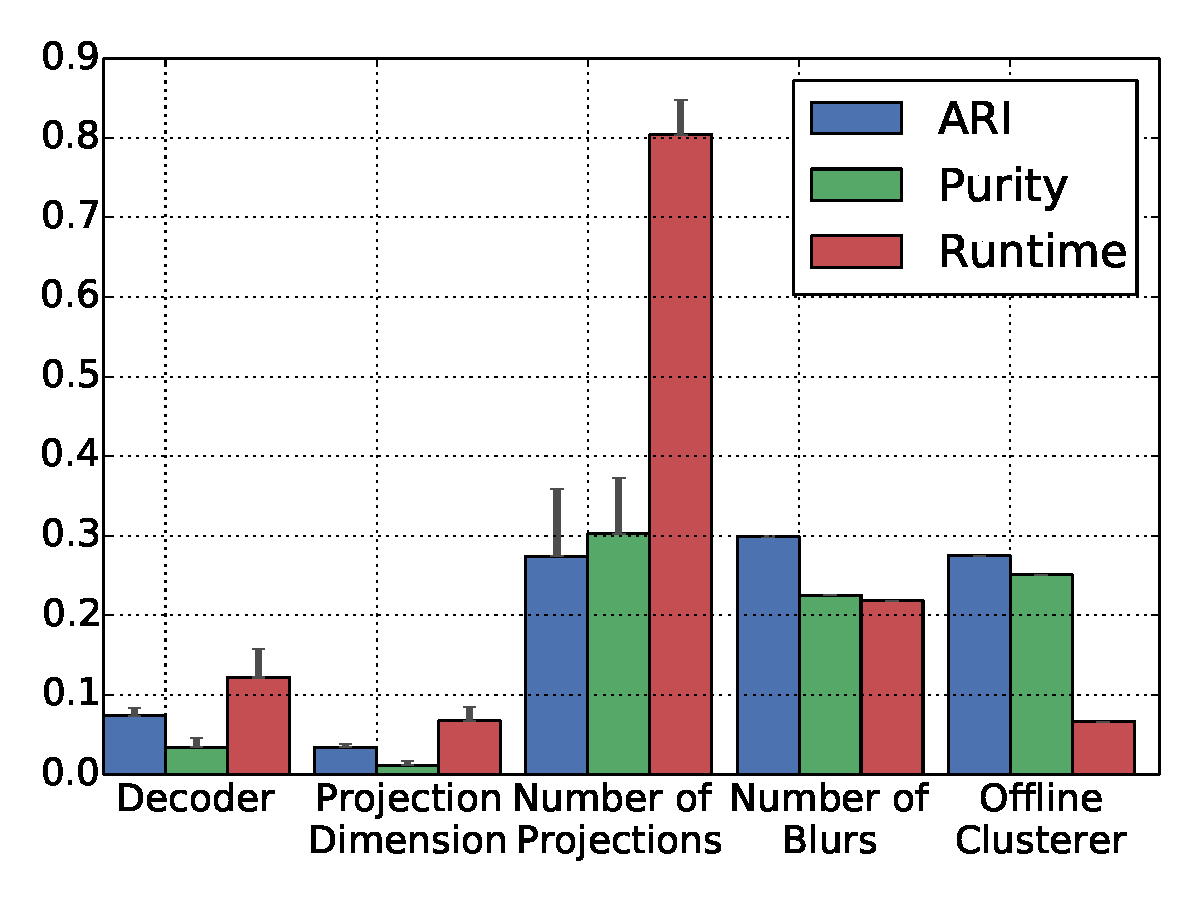
\includegraphics[width=.8\textwidth]{figs/correlation}}
  \caption{VIP analysis PLS regression results for 6400 configurations of \textsf{RPHash} on 7
    datasets.}\label{PLSreg}
\end{figure*}

\section{RPHash Performance}

Our first performance analysis section validates the performance of \textsf{RPHash} over a set of Real world
datasets followed by an analysis on synthetic datasets to validate the scalability of \textsf{RPHash}.  In
addition we give a detailed overview of clustering performance for various LSH functions available
for \textsf{RPHash} including our new Adaptive LSH.

\subsection{Experimental Approach}\label{experiments}
To assure \textsf{RPHash}'s accuracy and performance, tests for similarity to the standard clustering
algorithms, on various real and synthetic datasets are performed.  The experimental approach for
testing \textsf{RPHash} will address several major areas of \textsf{RPHash}'s utility, namely: (i)
Synthetic Algorithm Accuracy, (ii) Real World Data Set Accuracy, and (iii) Overall Scalability.

A required analysis of any $k$-means algorithm is its ability to correctly cluster expert labeled
data.  It is imperative that \textsf{RPHash} perform comparable to the standard clustering algorithms
in regard to external clustering accuracy metrics before timing and memory metrics are considered.
To evaluate the real world performance of \textsf{RPHash} with the optimal Leech based configuration
(Section \ref{optimalconf}), we clustered seven different datasets and compared the results to those
produced by six other well established clustering algorithms.  The R implementations used for the
six other clustering algorithms are listed in Section \ref{clusteralgos}.  In this test, we excluded
$k$-means$++$ due to it not offering significantly better results than standard $k$-means.

For each of the seven datasets, ground-truth partitions are known \emph{a priori}.  The ground-truth
labels are compared with labels produced by each clustering algorithm to compute the values of three
different external measures of clustering validation metrics are provided, \emph{Adjusted Rand
  Index} (ARI) and \emph{Cluster Purity} (see Section \ref{evalmetrics} for details).

The results are given in Table \ref{compareOtherAlgo} for ARI, Purity, Runtime, and Memory consumption.
Memory and Runtime performance are presented are averaged for each algorithm (`user time' in R) and
elapsed system time in Java, running on a computer configured with an Intel(R) Core(TM) i7-4770 CPU
with 4 cores @ 3.40GHz supporting 8 hardware threads and 32 GB memory. In these data sets we see that
\textsf{RPHash} performs, on average below standard $k$-means and similar to Ward's Method agglomerative. \textsf{RPHash} performs
better than the other linkage agglomerative clustering methods, and SOTA. \textsf{RPHash} outperforms
all other methods in regard to processing time and memory requirement by a large margin.  \textsf{RPHash} also
demonstrates a significant scalability advantage over the other methods.

\subsection{Performance Comparison}

\begin{table*}
\centering
\resizebox{\columnwidth}{!}{%
\begin{tabular}{|c|c|c|c|c|c|c|c|c|}
\hline
\rowcolor[HTML]{FFFFC7} 
\textbf{Data Set} & \textbf{Measures} & \cellcolor[HTML]{D1FF99}\textbf{\textsf{RPHash}} &
  \textbf{$k$-means} \cite{Hartigan} & \textbf{Single} & \textbf{Complete} & \textbf{Average} &
  \textbf{Ward's} & \textbf{SOTA} \cite{Herrero} \\ 
\rowcolor[HTML]{FFFFC7}
& & & & \textbf{Linkage} & \textbf{Linkage} & \textbf{Linkage} & \textbf{Method} \cite{Murtagh} &  \\ \hline
 & ARI     & 0.0697 &     0.0811 &    0.0461 &    0.0963 &    0.0546 &    0.0889 &    0.0981 \\
 & Purity  & 0.6058 &     0.6069 &    0.5730 &    0.5885 &    0.5752 &    0.5951 &    0.6062 \\
 & Runtime & 0.2709 &     0.5287 &    0.1680 &    0.1640 &    0.1680 &    0.1680 &    3.4440 \\
\multirow{-4}{*}{Arrhythmia}
 & Memory  & 0.7070 &    16.4333 &    3.4000 &    3.4000 &    3.4000 &    3.4000 &   21.3000 \\ \hline
 & ARI     & 0.2788 &     0.2798 &    0.0000 &    0.0000 &    0.0000 &    0.3547 &    0.1730 \\
 & Purity  & 0.4873 &     0.5312 &    0.1185 &    0.1204 &    0.1185 &    0.5722 &    0.3657 \\
 & Runtime & 0.3932 &     2.7120 &    4.3360 &    4.3400 &    4.3400 &    4.3440 &    3.7080 \\
\multirow{-4}{*}{CNAE-9}
 & Memory  & 1.1370 &   165.1167 &   24.2000 &   24.2000 &   24.2000 &   24.1000 &  134.2000 \\ \hline
 & ARI     & 0.0915 &     0.1158 &    0.0001 &    0.0120 &    0.0002 &    0.0930 &    0.0647 \\
 & Purity  & 0.3858 &     0.4271 &    0.3039 &    0.3335 &    0.3039 &    0.4597 &    0.3342 \\
 & Runtime & 0.8290 &    52.4100 &   71.9200 &   71.9600 &   71.9400 &   71.9720 &   11.7120 \\
\multirow{-4}{*}{Cora}
 & Memory  & 1.4590 &   227.9833 &  100.7000 &  100.7000 &  100.7000 &  100.7000 &  265.4000 \\ \hline
 & ARI     & 0.1282 &     0.0615 &    0.0000 &    0.0000 &    0.0000 &    0.0018 &    0.1147 \\
 & Purity  & 0.6720 &     0.6241 &    0.5001 &    0.5003 &    0.5001 &    0.5216 &    0.6694 \\
 & Runtime & 2.7363 &   423.7660 & 2280.4320 & 2280.4640 & 2280.0800 & 2280.5480 &   46.8120 \\
\multirow{-4}{*}{Gisette}
 & Memory  & 1.4300 &  2138.3833 &  829.3000 &  829.3000 &  829.3000 &  829.3000 & 2097.5000 \\ \hline
 & ARI     & 0.3348 &     0.4610 &    0.0000 &    0.3270 &    0.3321 &    0.4909 &    0.3143 \\
 & Purity  & 0.4631 &     0.6002 &    0.1890 &    0.3770 &    0.3588 &    0.6597 &    0.3966 \\
 & Runtime & 1.8774 &    24.7460 &  413.8800 &  414.3320 &  414.0960 &  414.4480 &   14.2440 \\
\multirow{-4}{*}{HAR}
 & Memory  & 0.5157 &  1485.0667 & 1259.0000 & 1214.9000 & 1214.8000 & 1214.9000 &  946.2000 \\ \hline
 & ARI     & 0.5043 &     0.6954 &    0.0001 &    0.0001 &    0.0001 &    0.6021 &    0.3351 \\
 & Purity  & 0.7105 &     0.7750 &    0.4635 &    0.4635 &    0.4635 &    0.7732 &    0.6918 \\
 & Runtime & 2.6363 &    23.8213 & 1093.9440 & 1094.7000 & 1094.8200 & 1095.5360 &   16.1880 \\
\multirow{-4}{*}{UJIIndoorLoc}
  & Memory  & 0.2460 & 2850.6500 & 5132.4000 & 5049.0000 & 5049.0000 & 5049.0000 & 2227.0000 \\ \hline
  & ARI     & 0.3205 &    0.4403 &    0.0066 &    0.0404 &    0.0066 &    0.3276 &    0.3906 \\
  & Purity  & 0.7063 &    0.7528 &    0.4755 &    0.5283 &    0.4755 &    0.7094 &    0.7019 \\
  & Runtime & 0.1648 &    0.8087 &    0.3760 &    0.3760 &    0.3760 &    0.3760 &    2.5400 \\
\multirow{-4}{*}{WebKB}
 & Memory  & 1.2000 &    50.1500 &    6.3000 &    6.4000 &    6.3000 &    6.3000 &   44.1000 \\ \hline
\end{tabular}
}
\caption{Comparison of Optimal Configuration of \textsf{RPHash} with Other Algorithms on Real World
  Datasets}\label{compareOtherAlgo}  
\end{table*}

\subsection{Adaptive LSH}

An extension to our initial \textsf{RPHash} work was the addition of the adaptive LSH decoder.  While this
decoder was not optimal, it is still an interesting result of this work.  In this experiment we
generated a synthetic dataset consisting of 10 Gaussian cluster uniformly distributed in 1000
dimensional space.  We then vary the inter-cluster variance of the clusters from 0 to 2.  The results
are shown in Figure \ref{twrpvothers}.  The blue line is the ground truth WCSSE, while the dashed
lines are Two-Pass \textsf{RPHash} with Leech Lattice Decoder, Two-Pass \textsf{RPHash} with the spherical (32,2,1)
decoder, and Two-Pass \textsf{RPHash} with Adaptive LSH.  This figure confirms the main results of our optimal
configuration experiment, while suggesting that Adaptive LSH may not be the best solution to the
space utilization problem discussed in Section \ref{adaptivespace}

\begin{figure}
     \centering
     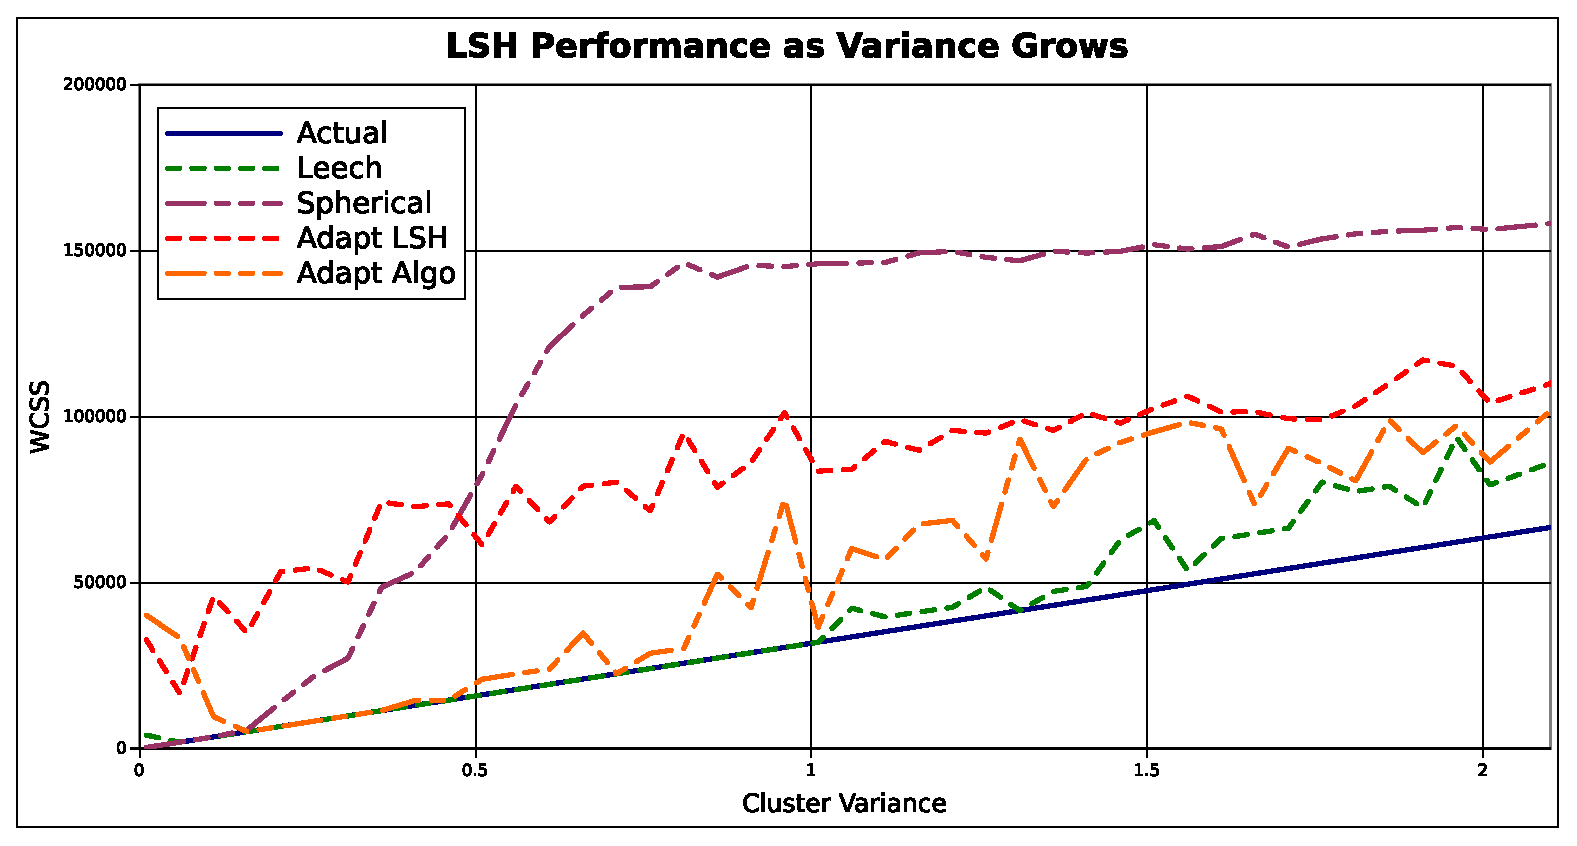
\includegraphics[width=.7\linewidth]{figs/clustervarianceVsDecoders} 
      \caption{Decoders Comparison on Varying Cluster Variance\label{twrpvothers}}
\end{figure}

\section{Streaming RPHash}

In this section, we evaluate the performance of \textsf{streamingRPHash} and compare it against
several other stream clustering algorithms, namely: Streaming $k$-means \cite{braverman}
implementation from S-Space \cite{sspace}, Damped Sliding Window \cite{zhu}, DStream \cite{dstream}
and Biased Reservoir Sampling \cite{ccaggarwal} (described in Section \ref{streamingalgos}).

\textsf{streamingRPHash} uses the optimal configuration described in Section \ref{optimalconf}.  We
apply the stream clustering algorithms on both real-world and synthetic data streams and evaluate
their clustering results based on various external, internal and entropy based clustering validation
measures.  Runtime and memory usage of all algorithms are also captured on a computer having Intel
Xeon X5675 CPU with 6 cores @ 3.07GHz supporting 12 hardware threads.  The operating system is
Debian `stretch' (x86\_64), running on 28 GB memory.  In addition, we assess the impact of noise on
stream clustering algorithms by injecting noise points in synthetic data streams.  Finally, we
perform a preliminary comparison of parallelization of \textsf{streamingRPHash} against streaming
$k$-means.  The results are described in the following subsections.

\subsection{Real-World Datasets}

\begin{figure*}
  \centerline{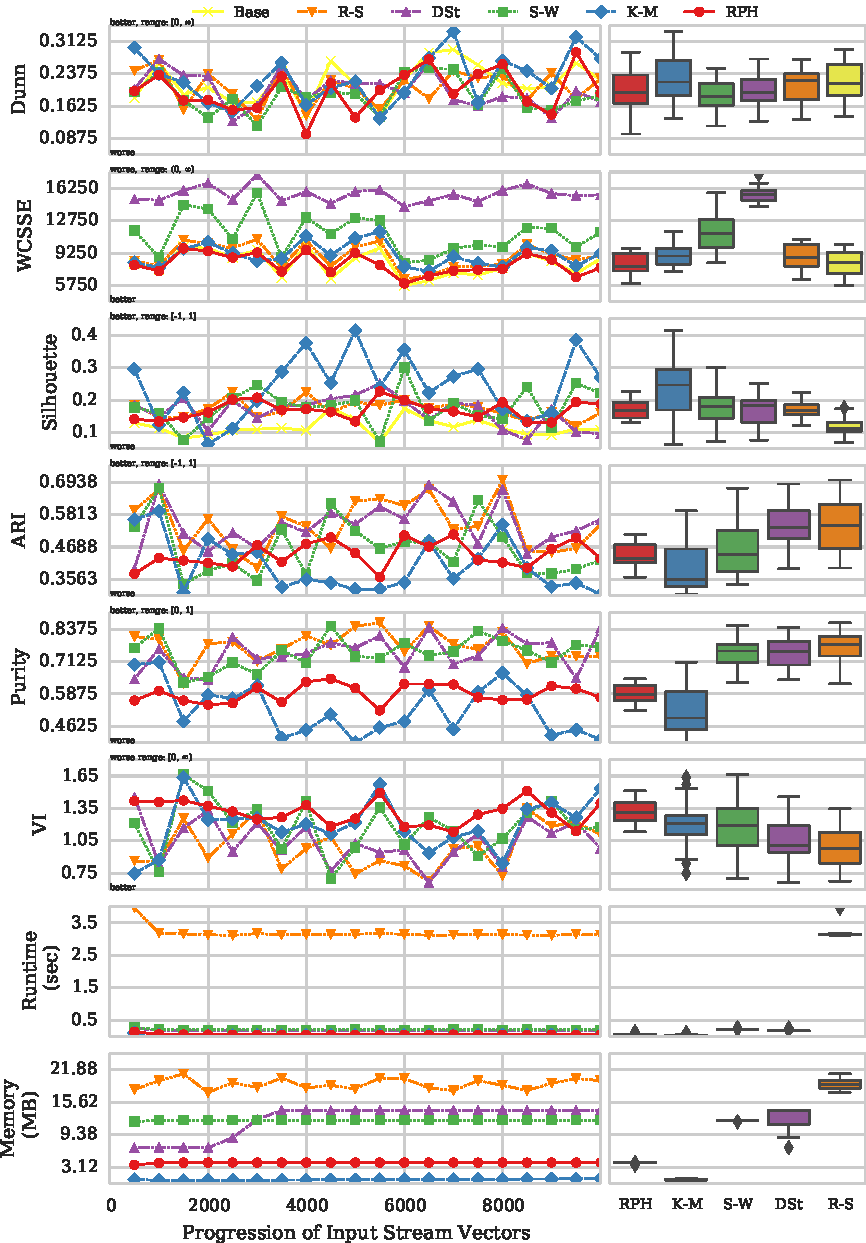
\includegraphics[width=.9\textwidth]{figs/har_all_measures}}
  \caption{Clustering Smartphone Sensor Data Comparison}{Clustering Results from Smartphone Sensor Data (abbreviations:
    RPH $\rightarrow$ \textsf{streamingRPHash},
    K-M $\rightarrow$ Streaming $k$-means,
    S-W $\rightarrow$ Damped Sliding Window,
    DSt $\rightarrow$ DStream,
    R-S $\rightarrow$ Biased Reservoir Sampling, and
    Base $\rightarrow$ Base Value}\label{human-measures}
\end{figure*}

\begin{figure*}
  \centerline{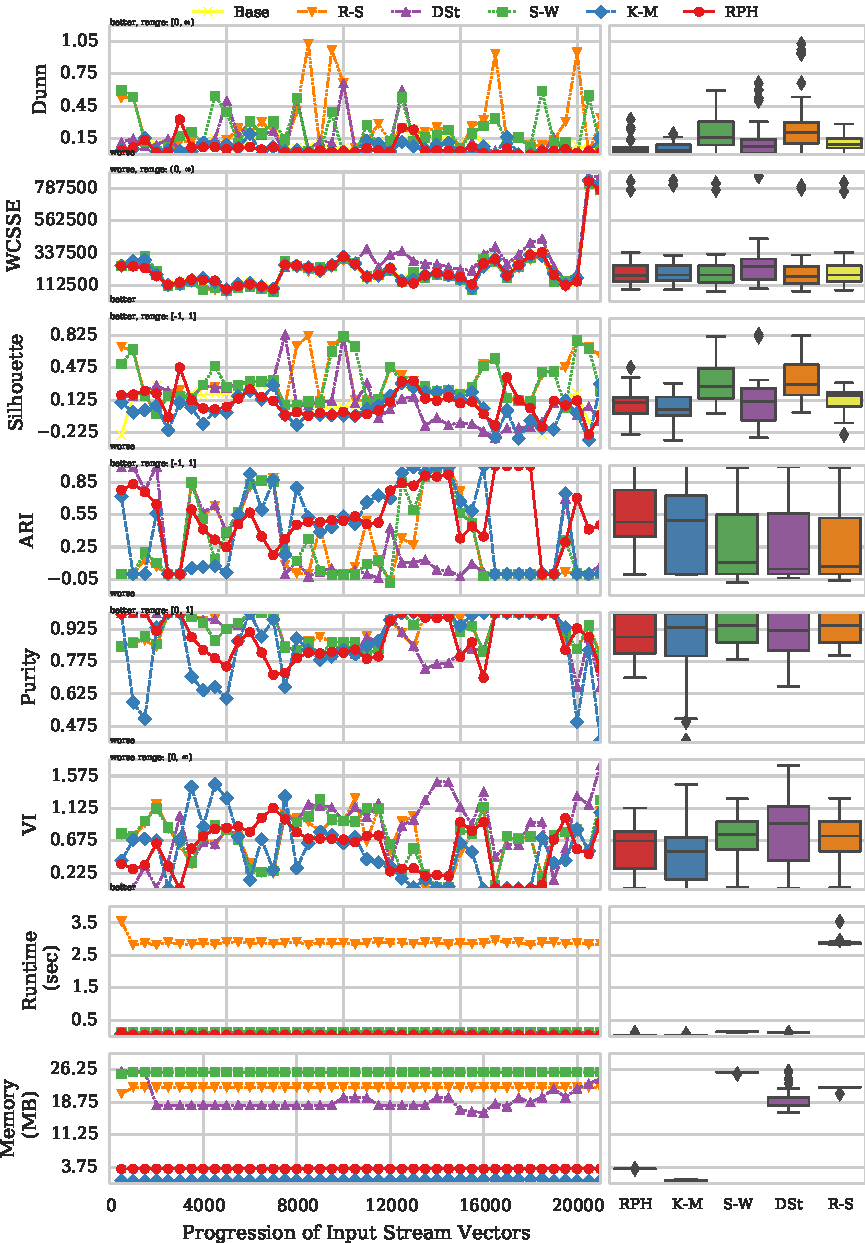
\includegraphics[width=.9\textwidth]{figs/ujii_all_measures}}
  \caption{Clustering Results from WiFi Location Data}{Clustering Results from WiFi Location Data (abbreviations:
    RPH $\rightarrow$ \textsf{streamingRPHash},
    K-M $\rightarrow$ Streaming $k$-means,
    S-W $\rightarrow$ Damped Sliding Window,
    DSt $\rightarrow$ DStream,
    R-S $\rightarrow$ Biased Reservoir Sampling, and
    Base $\rightarrow$ Base Value}\label{indoor-measures}
\end{figure*}

The algorithms are set up to report clustering results in batches of 500 points.  Performance
results for the \emph{HAR} dataset are shown in Figure \ref{human-measures}.  The plots are
organized into two side-by-side graphs.  The left graph shows the computed values at each 500 points
interval and the right graph is a box and whisker plot that shows the median and quartiles of all of
the sample points for each algorithm.  The results show that \textsf{streamingRPHash} performs on
par with the other algorithms.  The runtime performance is better than most and on par with
streaming $k$-means.  The memory usage is slightly worse than streaming $k$-means, but both are
significantly better (less than half) than the other algorithms studied.

The second dataset is the \emph{UJIIndoorLoc Data Set}\cite{UJII}.  Results from this dataset
are shown in Figure \ref{indoor-measures}.  The plots have the same format as with the previous
study.  Again, the clustering accuracy of \textsf{streamingRPHash} is on par with the other
algorithms while streaming $k$-means is the fastest and has a considerably smaller memory footprint.

\subsection{Scalability Study}

We study the dimensional scalability of stream clustering algorithms by evaluating their clustering
results as the dimensionality of data streams increases.  The purpose of this study is to assess and
compare the accuracy, runtime, and memory usage of \textsf{streamingRPHash} to those of other stream
clustering algorithms with increasing dimensionality.  Labeled data streams of 20,000 points and 10
randomly placed clusters with random multivariate Gaussian distributions are generated using the R
generator (as described in Section \ref{synth_data}).

The dimensionality of data streams, which increases in a sequence from 100 to 5767, follows two
polynomial sequences of the form $d_n = 1.5d_{n-1}$.  The first sequence starts from $d_0 = 100$ and
the second one from $d_0 = 125$.  We do not inject noise points or outliers in these data streams as
we inspect the impact of noise in the next section.  The clustering validation measures are computed
in batches of 1000 points and are plotted against dimensions of data streams.  For ease and clarity
of viewing the WCSSE plot, its values are scaled by diving by the number of dimensions.

Figures \ref{scalability-measures} and \ref{scalability-perf} show the performance results from this
scalability study.  The colored lines in each of these plots represent the mean value and shaded
regions around the lines represent the variance of a measure over all the batches of data points.
The shaded regions on the plots for DStream are wide and clearly visible as its measures have
significantly higher variances than those of other algorithms. In regard to clustering performance, \textsf{streamingRPHash}
performs optimally on all metrics with only one slight variation at 633 dimensions.  This performance
is on par with the other window and sampling streaming clustering algorithms, and outperforms
both DStream and streaming $k$-means.  The Runtime and memory requirements show a different story 
for Reservoir Sampling and Sliding window. Both of these algorithms require significantly more
processing time and space, with significantly worse growth complexity.  This plot shows a major strength
of \textsf{streamingRPHash}, in that it achieves near optimal clustering in linear processing time similar
to streaming $k$-means.

\begin{figure*}
  \centerline{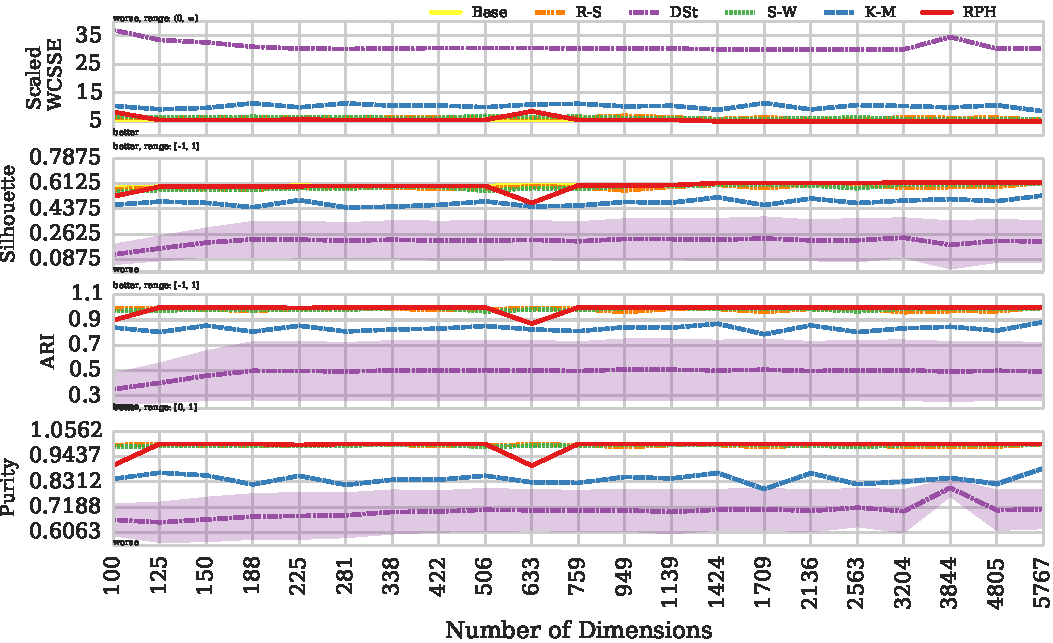
\includegraphics[width=1.1\textwidth]{figs/measure_scale}}
 \caption{Scaling Comparisons External and Internal Measures}{External and Internal Measures from Scaling the Number of Attributes (abbreviations: 
    RPH $\rightarrow$ \textsf{streamingRPHash},
    K-M $\rightarrow$ Streaming $k$-means,
    S-W $\rightarrow$ Damped Sliding Window,
    DSt $\rightarrow$ DStream,
    R-S $\rightarrow$ Biased Reservoir Sampling, and
    Base $\rightarrow$ Base Value}\label{scalability-measures}
\end{figure*}

\begin{figure*}
  \centerline{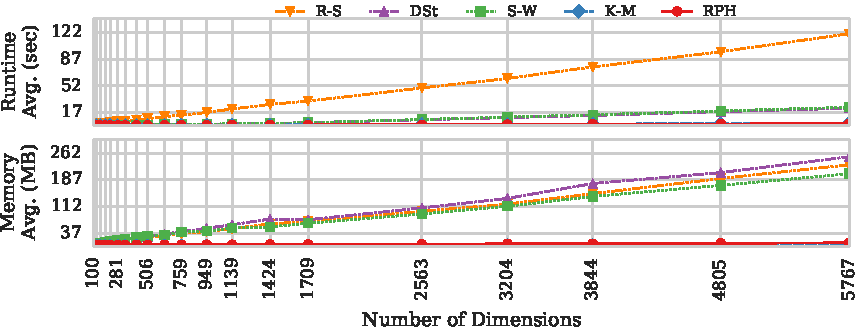
\includegraphics[width=.9\textwidth]{figs/runtimeGraphs}}
  \caption{Runtime and Memory usage from Scaling}{Runtime and Memory usage from Scaling the Number of Attributes (abbreviations:
    RPH $\rightarrow$ \textsf{streamingRPHash},
    K-M $\rightarrow$ Streaming $k$-means,
    S-W $\rightarrow$ Damped Sliding Window,
    DSt $\rightarrow$ DStream,
    R-S $\rightarrow$ Biased Reservoir Sampling, and
    Base $\rightarrow$ Base Value}\label{scalability-perf}
\end{figure*}

\subsection{Impact of Noise}\label{noise}

\begin{figure*}
  \centerline{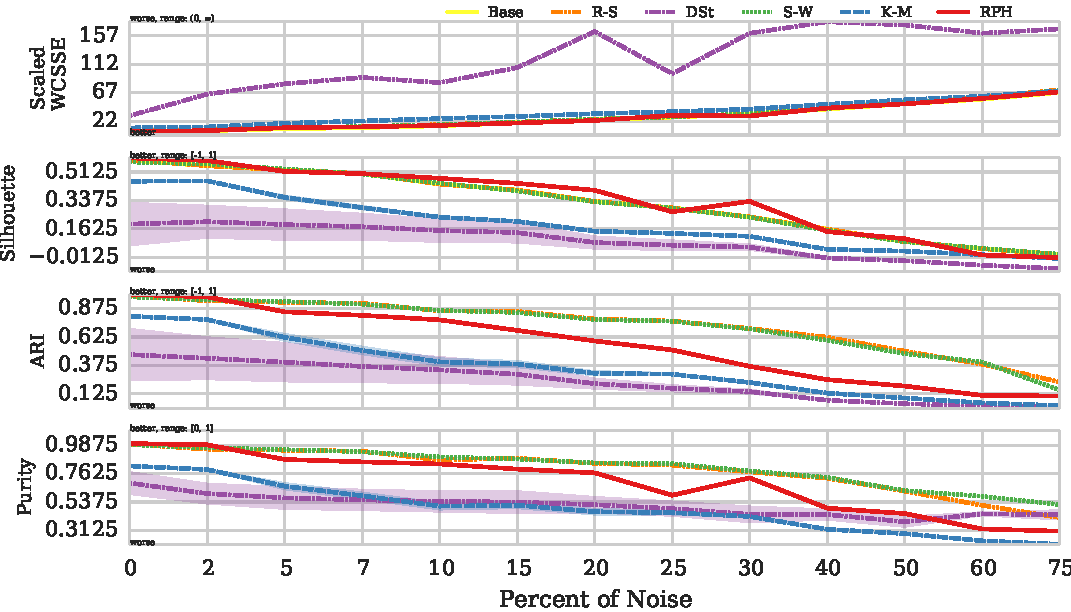
\includegraphics[width=1.1\textwidth]{figs/d759_noise}}
  \caption{Injecting Noise into the Data Source.}\label{noise-measures}
\end{figure*}

In this subsection, we assess the clustering results of \textsf{streamingRPHash} in the presence of
random noise in data streams.  We compare the clustering accuracy of \textsf{streamingRPHash} to
those of four other stream clustering algorithms while gradually increasing the percentage of noise
in a data stream.  We arbitrarily choose a dimension = 759 from those used for the scalability study
and generate several data streams with increasing amount of noise.  The percentage of random noise
is increased in an arbitrary sequence.  All of these noisy data streams are generated using the R
stream generator, where each data stream has 20,000 points and 10 randomly placed clusters with
random multivariate Gaussian distributions.  Noise points are assigned labels according to their
nearest cluster centroids.  We use the same clustering validation measures, same batch size (1000
points) and similar plots as with the scalability study.  The results are shown in Figure
\ref{noise-measures}.  The only difference here is that the horizontal axes represent percentage of
noise in data streams. In these figures we see that \textsf{streamingRPHash} performs optimally
in regard to the other algorithms and even baseline for WCSSE and Silhouette, as noise is injected. 
It performs mediocre in the two external metrics ARI and cluster Purity, besting streaming $k$-means 
and DStream.

\section{Tree-Walk RPHash Performance}

In this section we explore the clustering performance of the Tree-Walk RPHash variant (\textsf{TWRP}).  The
\textsf{TWRP} variant of \textsf{RPHash} is what we would consider our best of breed \textsf{RPHash} algorithm.  \textsf{TWRP} uses
information about the data distribution to build adaptive LSH functions, and also more thoroughly
explores the relationships between clusters and encapsulated clusters.  We first compare \textsf{TWRP} to
various other clustering algorithms on real world data, then we explore the scalability, and noise
robustness of \textsf{TWRP}.

\subsection{Real World Data} 
	
The largest and most stable dataset that we've explored so far is the \emph{Human Activity Recognition} dataset \cite{har} dataset.  
The attributes of this dataset are available in Table
\ref{realworld}.  We compare \textsf{TWRP} to standard \textsf{RPHash} as well as our usual set of standard clustering
algorithms, consisting various Agglomerative methods, standard $k$-means, and SOTA.  The results can
be found in Table \ref{perftimetable}.  We captured the runtime (in Secs) performance for all of the
algorithms and results were obtained on a computer with an Intel Core(TM) i7-4770 CPU with 4 cores @
3.40 GHz and 32 GB memory.  Among the compared algorithms \textsf{TWRP} improves upon the performance of standard
\textsf{RPHash} and performs on par with $k$-means and Ward's linkage agglomerative clustering.  The main
benefit however is in its timing results. \textsf{TWRP} is 100x faster than $k$-means, and 2000x faster
than Ward's linkage agglomerative clustering.

\begin{center}
 \begin{table*}
  \centering
\begin{tabular}{|c|c|c|c|c|}\hline
\cellcolor[gray]{0.9}\textbf{Algorithm}	&\cellcolor[gray]{0.9}\textbf{ARI}	&\cellcolor[gray]{0.9}\textbf{Purity} &\cellcolor[gray]{0.9}\textbf{WCSSE} &\cellcolor[gray]{0.9}\textbf{Time} \\ \hline
\cellcolor[gray]{0.9}\textbf{Kmeans}		&0.461  &0.6   &182168.7&24.746\\\hline
\cellcolor[gray]{0.9}\textbf{Single Link}  		&0      &0.189 &556519.1&413.88\\\hline
\cellcolor[gray]{0.9}\textbf{Complete Link}  		&0.327  &0.377 &222044.4&414.33\\\hline
\cellcolor[gray]{0.9}\textbf{Average Link}  		&0.332  &0.359 &236142.8&414.1\\\hline
\cellcolor[gray]{0.9}\textbf{Ward's}		&0.491  &0.66  &191441.1&414.45\\\hline
\cellcolor[gray]{0.9}\textbf{SOTA}  		&0.314  &0.397 &210490.1&14.244\\\hline
\cellcolor[gray]{0.9}\textbf{RPHash}		&0.363  &0.508 &210628.6&0.4838\\\hline
\cellcolor[gray]{0.9}\textbf{TWRP}	&0.449	&0.609 &194688.7&0.2617\\\hline
\end{tabular}
\caption{Clustering Performance and Timing}\label{perftimetable}
\end{table*}
\end{center} 

\subsubsection{Synthetic Data}

In this experiment we generated datasets with successive dimensionality in $\mathbb{R}^{100}$ to
$\mathbb{R}^{7000}$ space.  Each dataset consists of 10000 vectors equi-probable chosen from a set of
10 univariate Gaussian clusters.  Figures \ref{perfdim1},\ref{perfdim2},\ref{perfdim3} give the
clustering performance of \textsf{TWRP} compared to other clustering algorithms for the metrics, ARI , Purity
and WCSSE on the generated datasets.  \textsf{TWRP} performs optimally for all dimensions, equaling the agglomerative
methods.  It is also stable, compared to standard \textsf{RPHash} and $k$-means.


\begin{figure*}
    \centering
    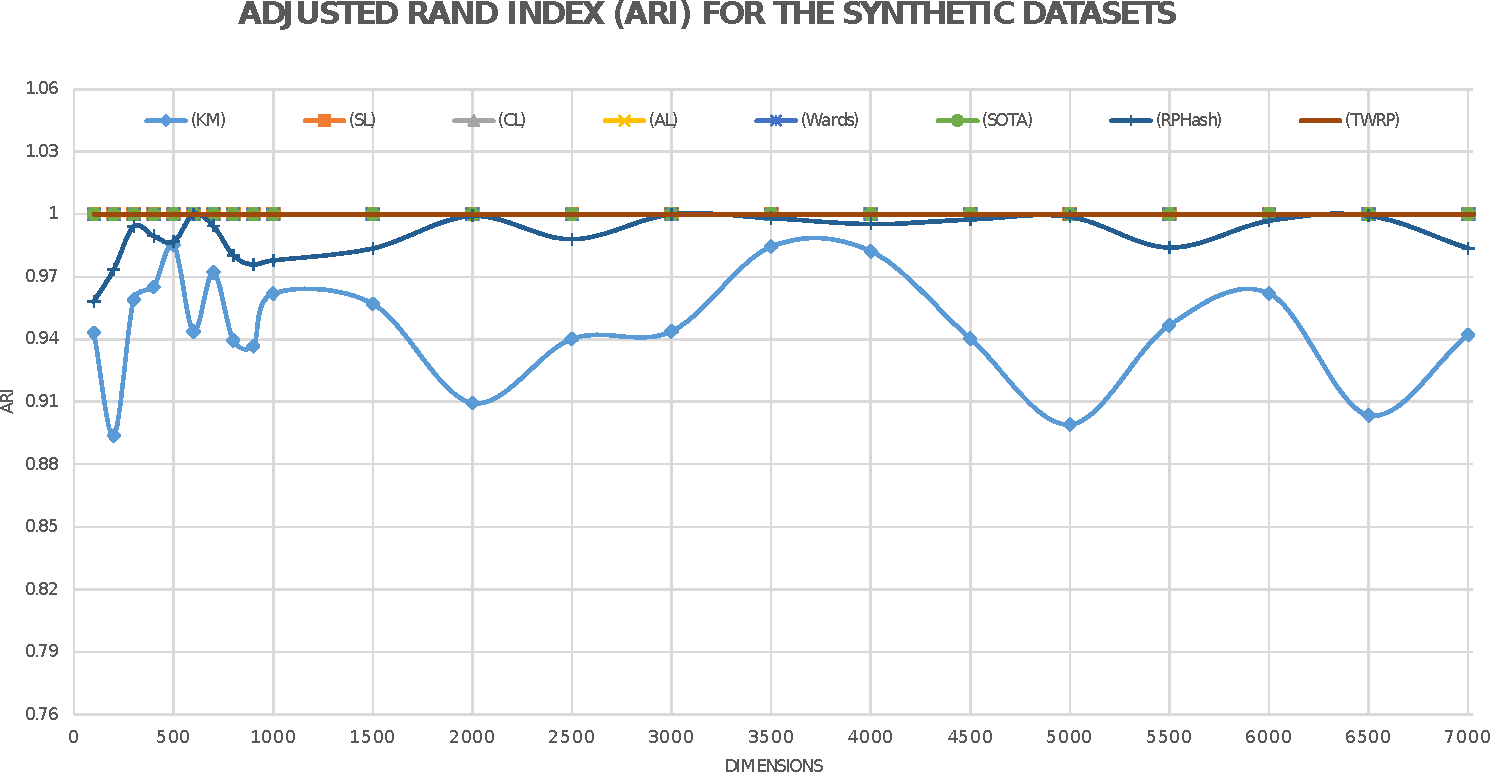
\includegraphics[width=1\linewidth]{figs/ari_synthetic_2} 
    \caption{ARI Synthetic} \label{perfdim1}
\end{figure*}
\begin{figure*}
    \centering
    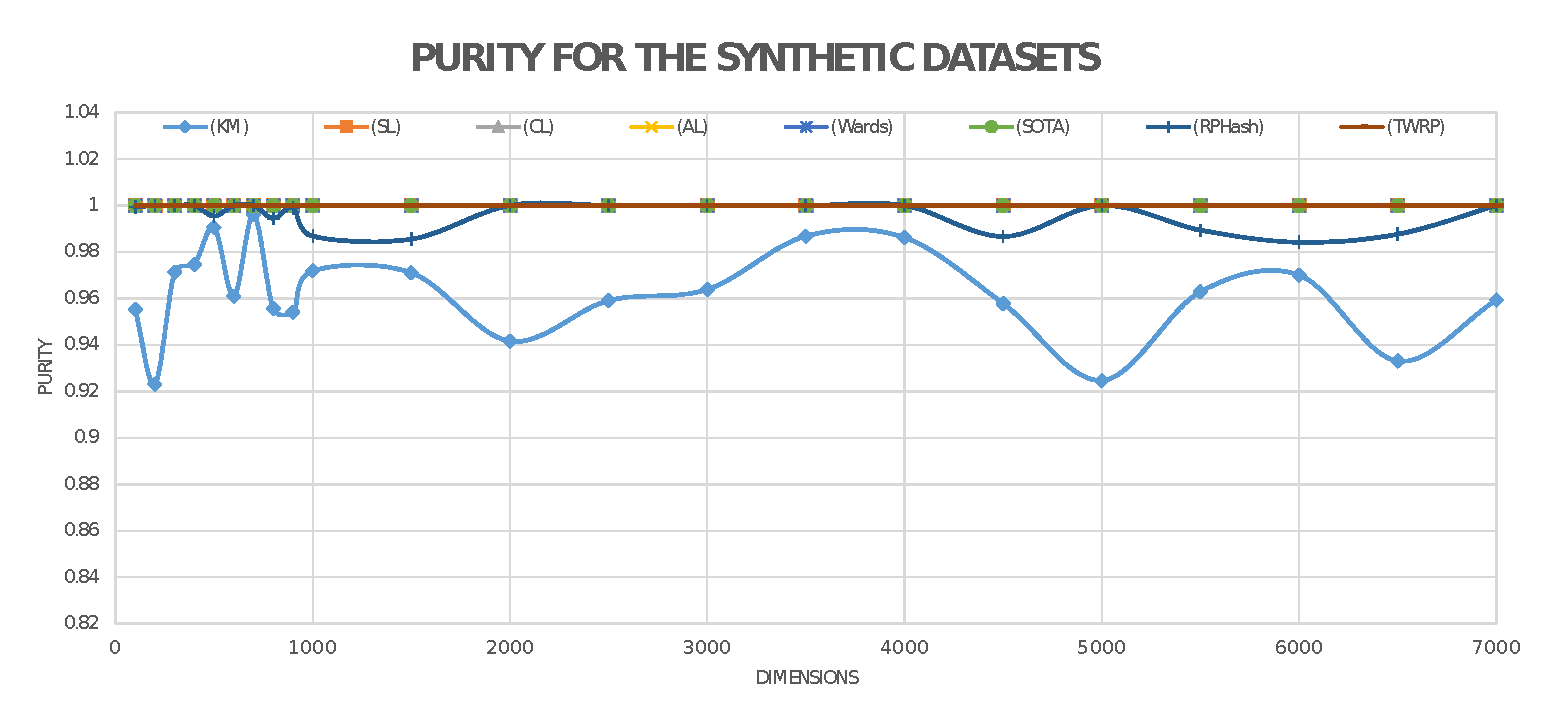
\includegraphics[width=1\linewidth]{figs/purity_synthetic_2} 
    \caption{Purity Synthetic} \label{perfdim2}
\end{figure*}
\begin{figure*}
    \centering
    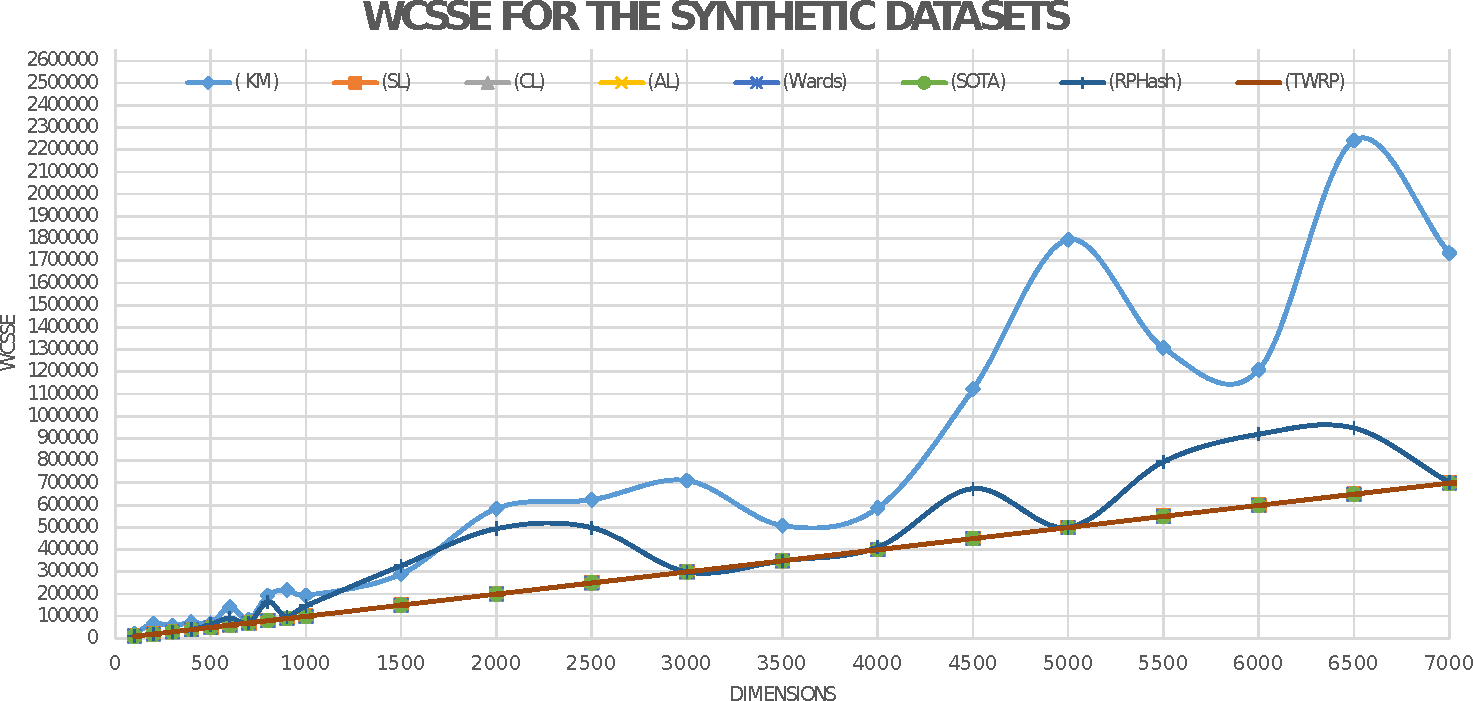
\includegraphics[width=1\linewidth]{figs/wcsse_synthetic_2} 
    \caption{WCSSE Synthetic}\label{perfdim3} 
\end{figure*}

\subsubsection{Noise Stability}

An important test of a clustering algorithm's versatility is its robustness to noise.  In general,
real world data will contain at least some level of noise due to systematic errors in measurement.
In this experiment we will generate datasets with varying amount of noise. We chose a dimensionality
of 1000 dimension and inject noise varying from 5 percent to 50 percent of the overall dataset size
in increments of 5 percent.  The noise vectors generated were assigned the label of the closest
cluster center.  The results of the noise injection tests are plotted in Figures
\ref{noiseacc1},\ref{noiseacc2},\ref{noiseacc3}, with ARI, Purity, and WCSSE being tracked
respectively.

\begin{figure*}
    \centering
    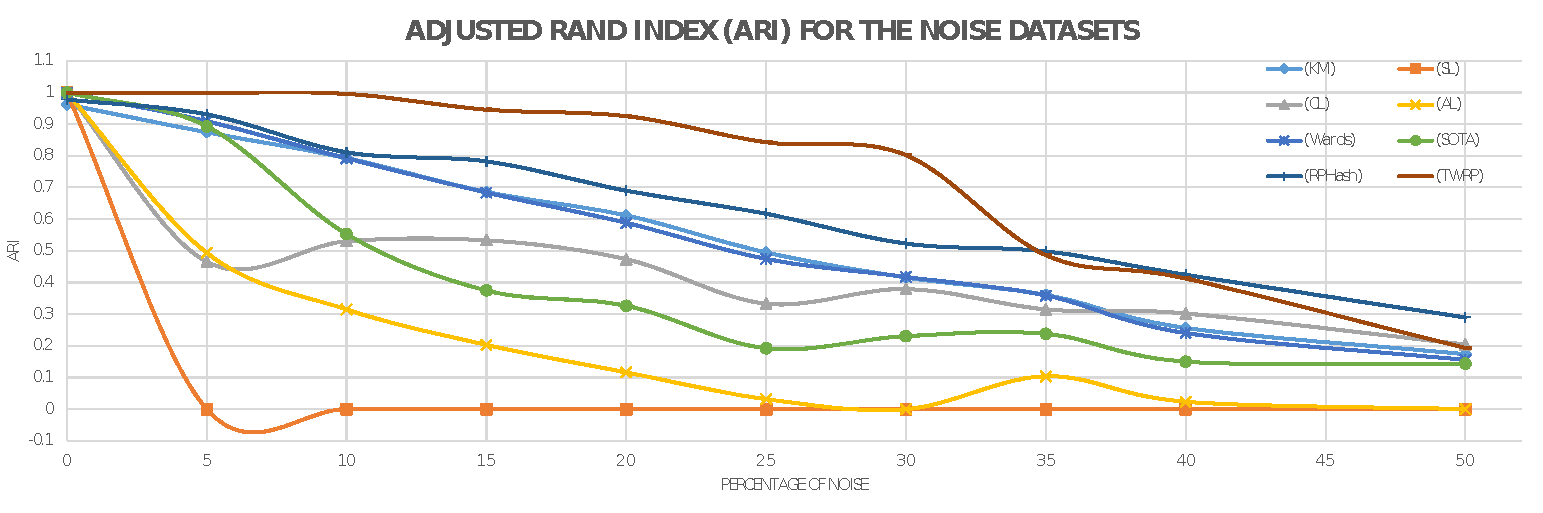
\includegraphics[width=1\linewidth]{figs/ari_noise_2} 
    \caption{ARI Noise}\label{noiseacc1} 
\end{figure*}
\begin{figure*}
    \centering
    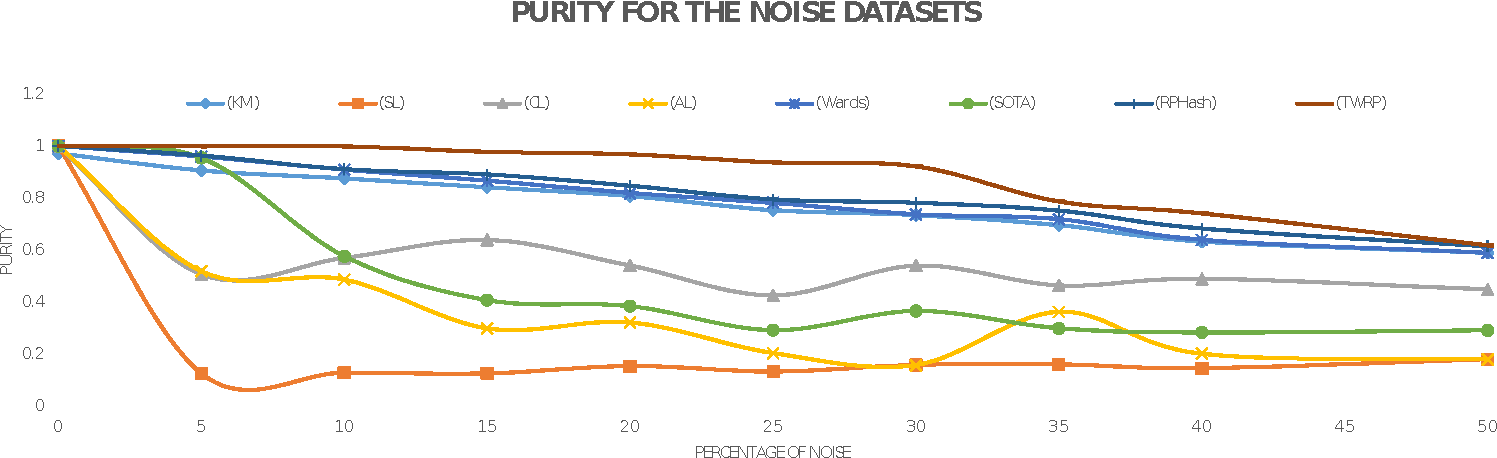
\includegraphics[width=1\linewidth]{figs/purity_noise_2} 
    \caption{Purity Noise}\label{noiseacc2} 
\end{figure*}
\begin{figure*}
    \centering
    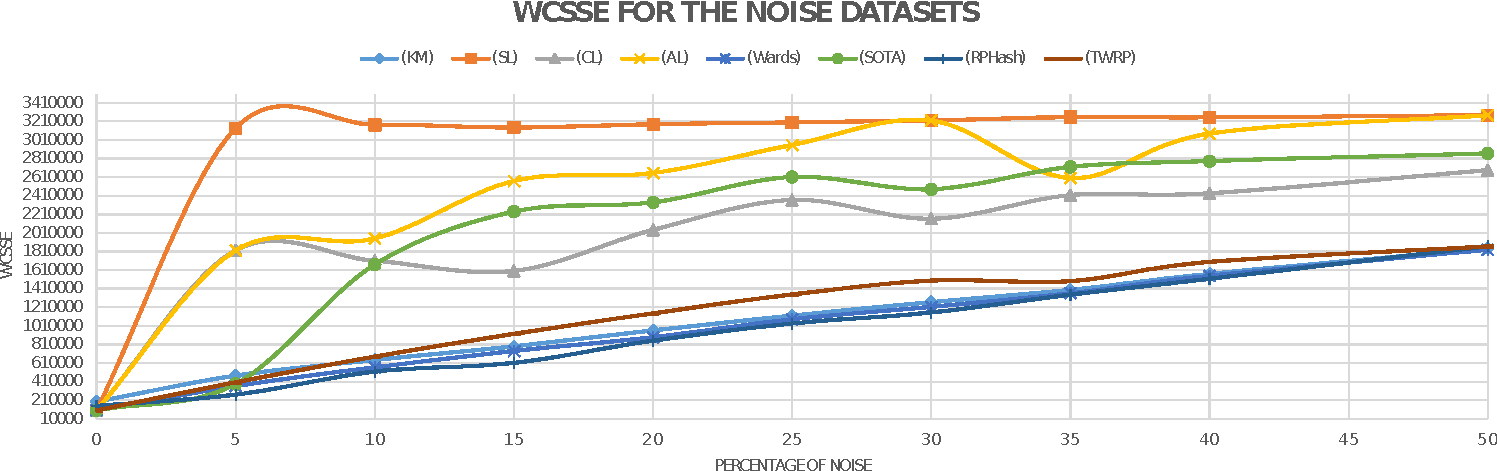
\includegraphics[width=1\linewidth]{figs/wcsse_noise_2} 
    \caption{WCSSE Noise}\label{noiseacc3} 
\end{figure*}

We observe that until the noise percentage reaches 40 the accuracy of both the \textsf{RPhash} algorithms
are far better than the other six standard algorithms. Thereafter as the noise grows beyond 50
percent and the signal to noise ratio is very low, all the algorithms tend to perform poorly.

\subsubsection{Scalability}

Table \ref{scalability} summarizes the timing results on synthetic datasets.  The data sets were
generated using the R data generator discussed in Section \ref{synth_data} to generate 10000 vectors from $k=10$
univariate clusters, with varying dimensionality.  Results for all clustering algorithm timings were
obtained on a computer with Intel(R) Xeon(R) E5-2670 @ 2.6 GHz with 16 cores and 64 GB RAM.  While
Table \ref{scalability} gives a detailed measure of the scalability for all comparison clustering
algorithms, Figure \ref{twrp_scale} shows difference between the \textsf{RPHash} algorithms and only the two
faster comparison clustering methods.  This is due to the agglomerative methods being so much slower
that they would skew the output plot making it useless for comparison.  In this experiment we see again
that the scalability of the \textsf{RPHash} algorithms far exceeds the other compared methods.  While SOTA and $k$-means
achieve, what appears to be linear complexity growth, the \textsf{RPHash} methods, appear constant in comparison.  This 
of course is not true and they share a similar linear complexity with  SOTA and $k$-means. We 
can verify this in the scalability Table \ref{scalability}, but should note that the difference in processing time, 
between \textsf{RPHash} algorithms, SOTA, and $k$-means is significant.

\begin{center}
 \begin{table*}
 \centering
\begin{tabular}{|c|c|c|c|l|l|}\hline
\cellcolor[gray]{0.9}\textbf{Dimension}&\cellcolor[gray]{0.9}\textbf{KMeans}&\cellcolor[gray]{0.9}\textbf{AverageLinkage}&\cellcolor[gray]{0.9}\textbf{SOTA}&\cellcolor[gray]{0.9}\textbf{RPHash}&\cellcolor[gray]{0.9}\textbf{TWRP}\\

\cellcolor[gray]{0.9}&\cellcolor[gray]{0.9}&\cellcolor[gray]{0.9}\textbf{Link}&\cellcolor[gray]{0.9}
\cellcolor[gray]{0.9}&\cellcolor[gray]{0.9}\textbf{Leech}&\cellcolor[gray]{0.9}\\\hline 

\cellcolor[gray]{0.9}\textbf{100}&3.9656&47.46&13.758&0.4890&0.1638\\\hline
\cellcolor[gray]{0.9}\textbf{300}&13.3796&194.121&23.797&0.4782&0.1638\\\hline
\cellcolor[gray]{0.9}\textbf{500}&32.92&454.777&36.046&0.5594&0.3005\\\hline
\cellcolor[gray]{0.9}\textbf{700}&77.7298&672.759&48.963&0.6174&0.3642\\\hline
\cellcolor[gray]{0.9}\textbf{900}&117.3675&929.6&61.759&0.7052&0.4078\\\hline
\cellcolor[gray]{0.9}\textbf{1000}&142.2341&1064.178&68.86&0.7206&0.4318\\\hline
\cellcolor[gray]{0.9}\textbf{1500}&237.0007&1789.142&96.795&0.8233&0.5392\\\hline
\cellcolor[gray]{0.9}\textbf{2000}&366.0743&2450.813&127.972&0.8796&0.6548\\\hline
\cellcolor[gray]{0.9}\textbf{2500}&431.5876&3108.654&155.968&0.9997&0.8050\\\hline
\cellcolor[gray]{0.9}\textbf{3000}&542.0223&3771.886&185.23&1.1122&0.8917\\\hline
\cellcolor[gray]{0.9}\textbf{3500}&631.8423&4435.349&220.562&1.2421&1.0229\\\hline
\cellcolor[gray]{0.9}\textbf{4000}&741.915&5080.802&248.669&1.3157&1.1498\\\hline
\cellcolor[gray]{0.9}\textbf{4500}&811.3911&5725.061&274.983&1.3986&1.2873\\\hline
\cellcolor[gray]{0.9}\textbf{5000}&909.223&6362.574&301.314&1.5095&1.4128\\\hline
\cellcolor[gray]{0.9}\textbf{5500}&975.2703&7006.91&324.314&1.5977&1.5392\\\hline
\cellcolor[gray]{0.9}\textbf{6000}&1076.882&7645.155&359.911&1.6805&1.6157\\\hline
\cellcolor[gray]{0.9}\textbf{6500}&1187.6062&8278.964&400.767&1.7933&1.7266\\\hline
\end{tabular}
\caption{Scalability Study.}\label{scalability}
\end{table*}
\end{center}

\begin{figure*}
    \centering
    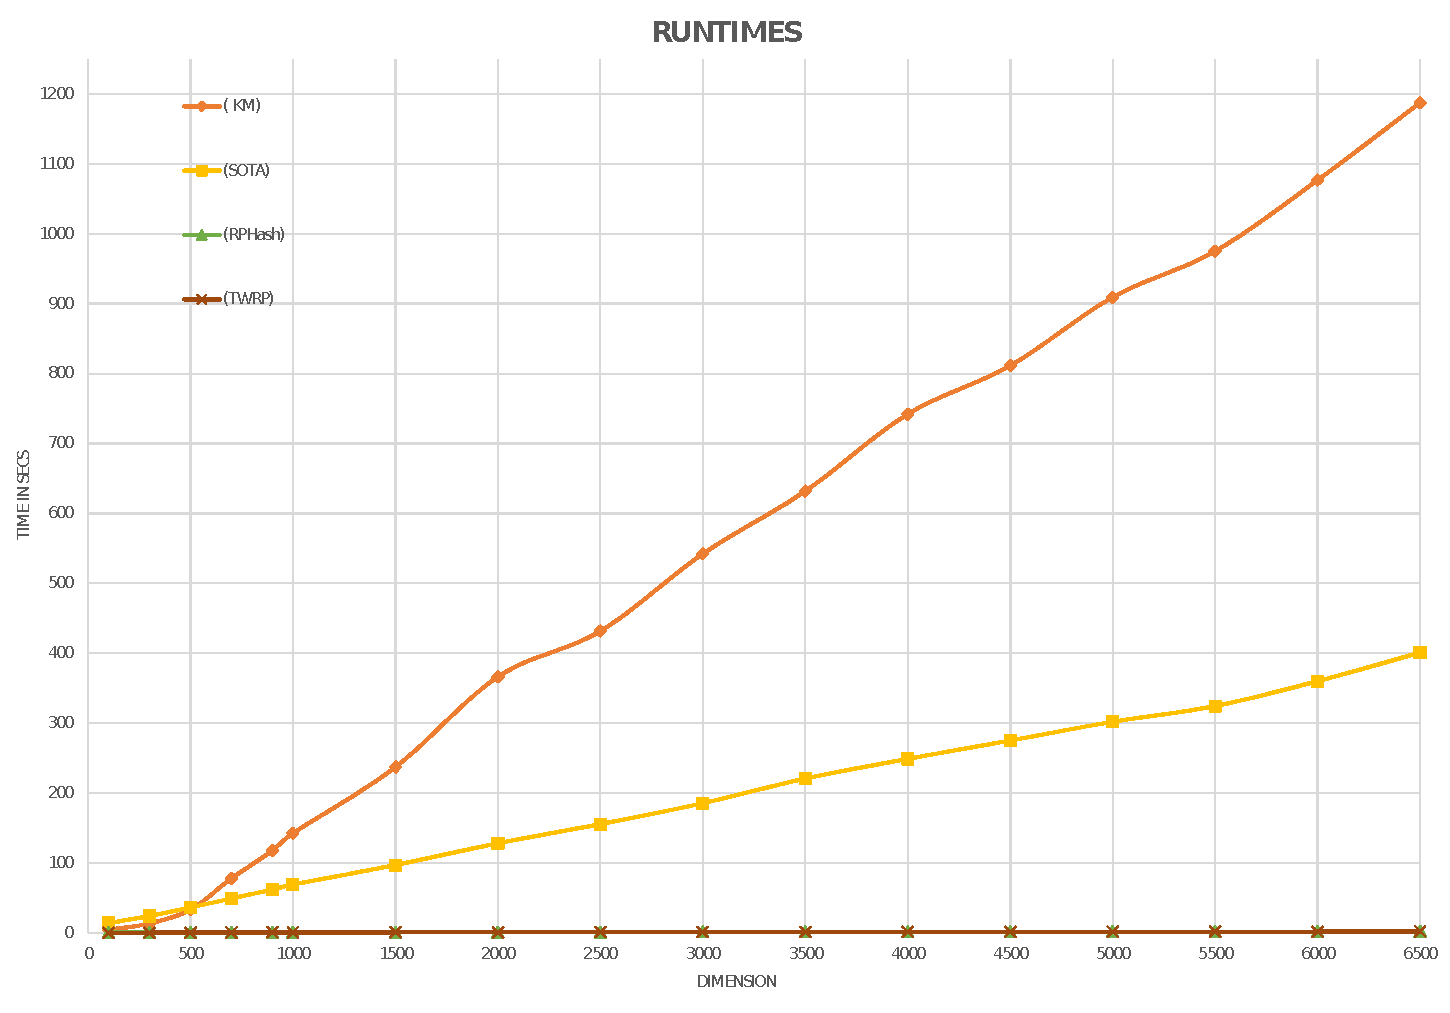
\includegraphics[width=.8\linewidth]{figs/Scalability_Synthetic} 
    \caption{SCALABILITY Synthetic}\label{twrp_scale}
\end{figure*}

\subsection{Tree Walk RPHash (\textsf{TWRP}) Results on Word2Vec Data}

In this section we used the GoogleNews \cite{googlenews} Word2Vec dataset to compare the clustering
and timing performance of \textsf{TWRP} with $k$-means++.  Word2Vec data is particularly interesting, because
it often contains very large, high dimensional, and dense, data vectors that often occupy lower
dimensional embeddings.  However, due to the size of the observations, it is unlikely that a ground
truth will be available.  Observation can verify certain subjective aspects of the data clustering,
such as two similar words or concepts being labeled in the same cluster, but an overall labeling is
usually unavailable.  For this experiment, we rely on the WCSSE only to act as a performance metric.
We could theoretically compute other external metrics, such as Silhouette and Dunn Index however
given the size of the GoogleNews data set, it is computationally infeasible.  In addition, we do not
have a defined number of clusters.  Figure \ref{w2vwcss} gives the WCSSE for a sequence of possible
values of $k$ for \textsf{TWRP} and $k$-means++.  Likewise, Figure \ref{w2vratio} gives the ratio of the
$k$-means++ WCSSE and \textsf{TWRP} WCSSE.  Under the assumption that $k$-means++ finds nearly the optimal
WCSSE, we can regard \textsf{TWRP} as an $\epsilon$-error equivalent.  As \textsf{TWRP} appears to be outperformed in
regard to WCSSE, by $k$-means++, it is important to focus on some of its advantages, namely its
speed.  Figure \ref{w2vproctime} gives a comparison of the two algorithms in regard to processing
time.  As, is clear in other runtime performance tests, the TWRP algorithm scales linearly with the
data size, and overall requires far less computation than $k$-means, and similar algorithms.

\begin{figure}[t]
        \centering
        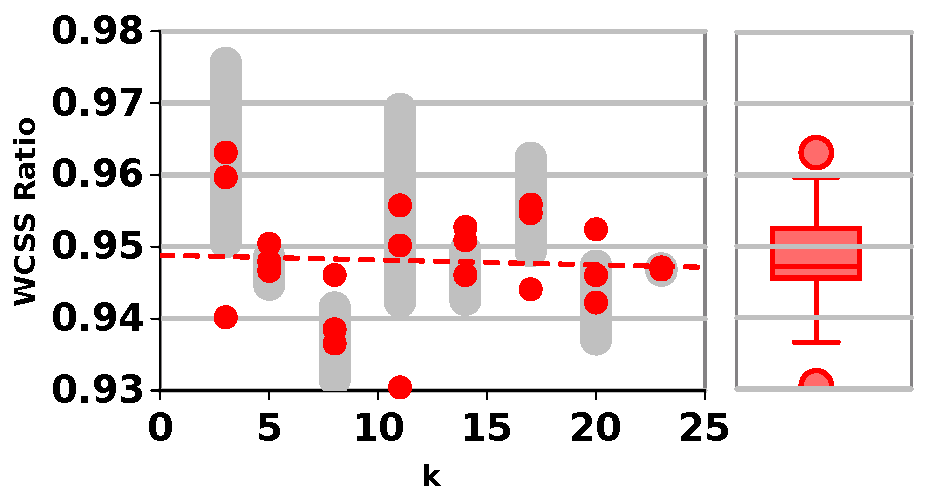
\includegraphics[width=.75\textwidth]{figs/w2vratio_wcss.pdf}
	\caption{WCSSE KMeans++ to \textsf{TWRP} Ratio}\label{w2vratio}
\end{figure}
\begin{figure}[t] 
        \centering
        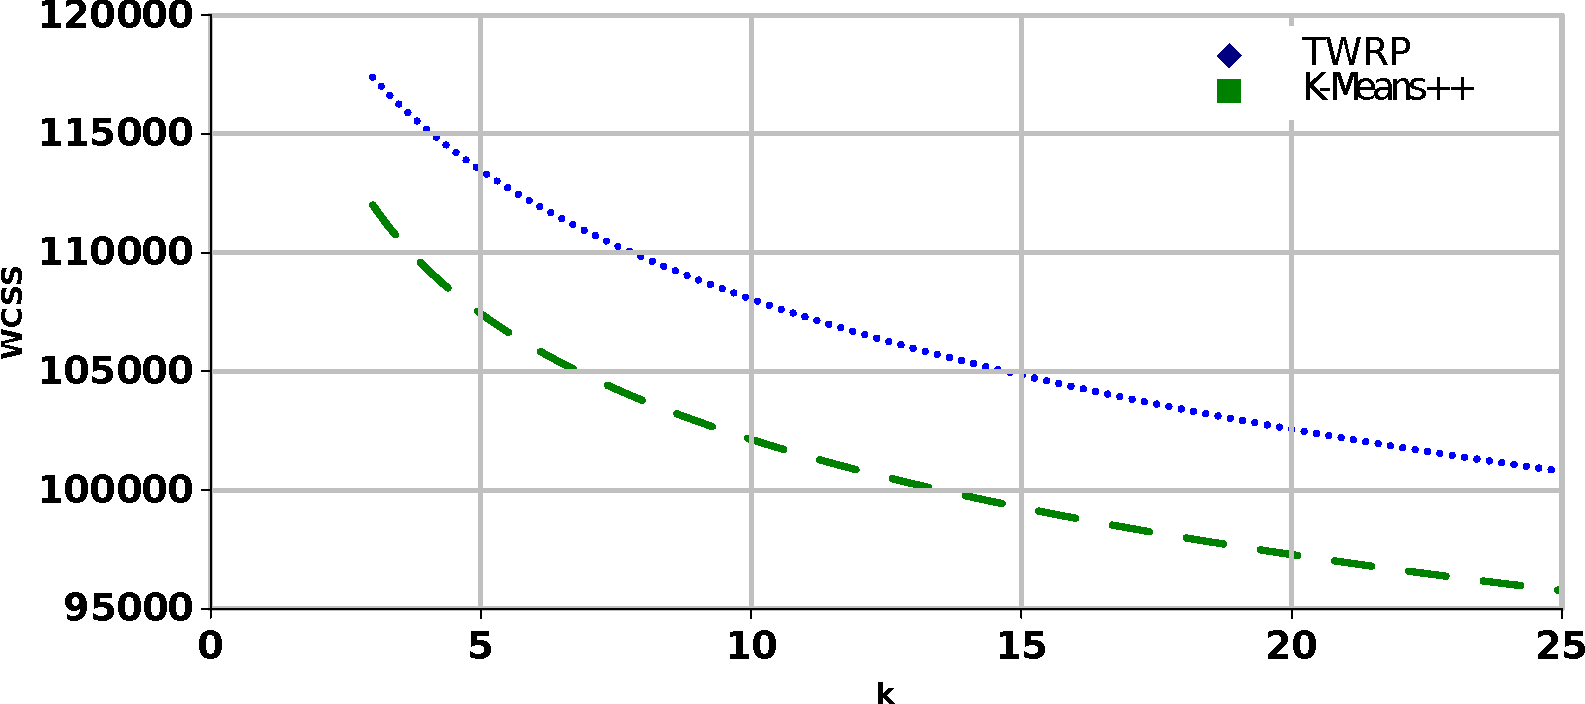
\includegraphics[width=.85\textwidth]{figs/w2vwcss.pdf}
	\caption{WCSSE Comparison Results}\label{w2vwcss}
\end{figure}
\begin{figure}[t]
        \centering
	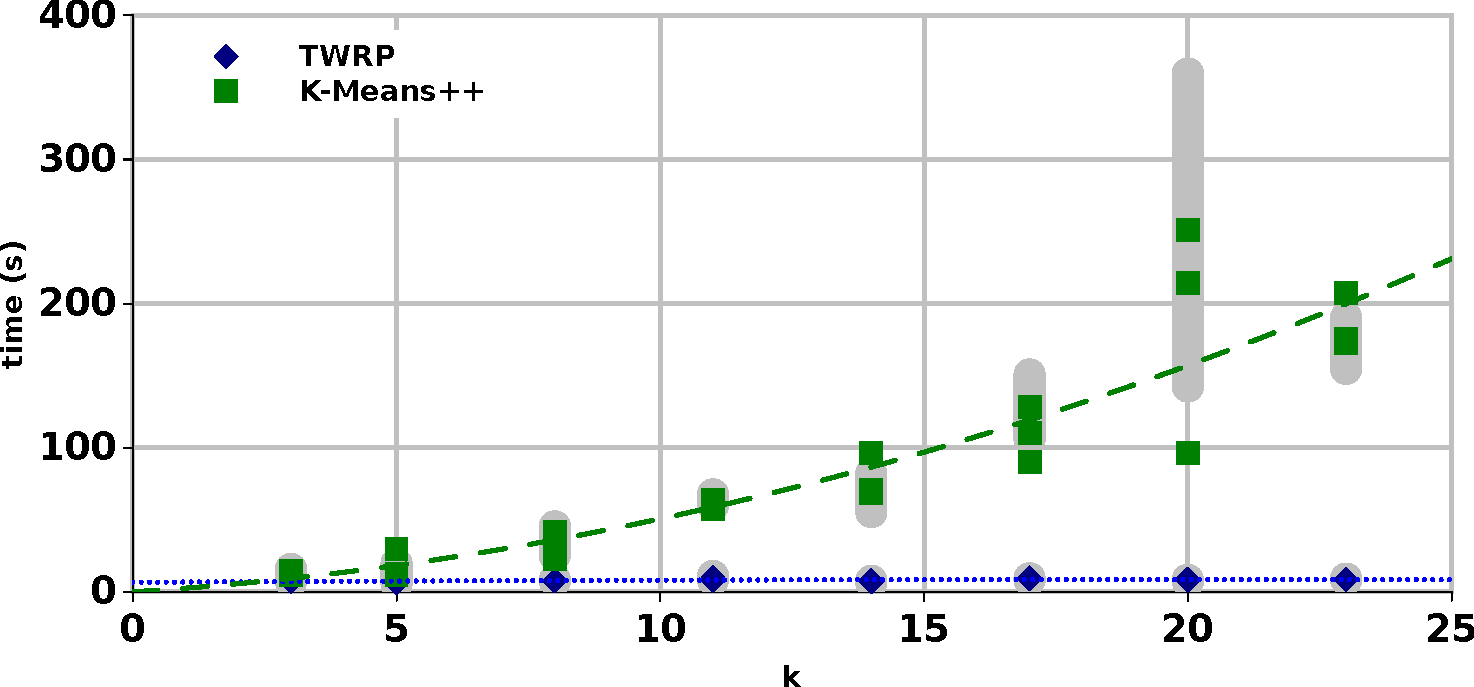
\includegraphics[width=.85\linewidth]{figs/w2vtime.pdf}
	\caption{Processing Time Comparison}\label{w2vproctime}
\end{figure}


\section{RPHash Parallelism}

\textsf{RPHash} was designed with the intent of being naively parallelizable.  As with many parallel
adaptations of well-known machine learning algorithms, the influence of Amdahl's Law appears during
parallelization efforts due to unavoidable sequential bottlenecks as the number of processing nodes
increases.

In this section we compare the three proposed variants of \textsf{RPHash} in regard to parallel speedup.  Our
testing was done on an 8-core Intel Xeon CPU with 4 threads per core, for a total of 32 sequential
threads.  The parallelism was implemented similar to our target platforms of map-reduce and spark
streaming interface.

\subsubsection{Standard RPHash}

The standard \textsf{RPHash} algorithm parallel implementation consists of an equal partitioning of vectors
to processing units.  In the map phase, each processing unit applied the per vector process to their
respective subset of vectors in parallel.  The threads then performed a log reduction sum of the
counts of hash collisions in the thread's respective subset of vectors. The result of the first
phase is a set of the densest hash bucket, IDs.  The second phase then proceeds byt redistributing
the data vectors to processing nodes, and accumulating a centroid for vectors that produce hashes
that collide with the dense set of hash bucket IDs. These centroids are then reduced through a
weighted sum log reduction of the centroids.

\subsubsection{TWRP}

The tree walk variant consists of a similar equal partitioning of vectors among processing nodes as
the standard \textsf{RPHash} variant.  Similarly, each node accumulates a separate MinCount data
structure.  Once all vectors have been processed, the MinCount structures are merged, for all
indices.  The result is the complete MinCount structure, from which the tree based, off-line step of
\textsf{TWRP} proceeds sequentially. In our tests, we only tested the sequential off-line step, however,
various parallel depth first search methods could be employed to improve performance and parallel
speedup.

\subsubsection{Streaming RPHash}

The \textsf{streamingRPHash} variant is discussed last because it differs the most from the previous
algorithms.  Namely, the \textsf{streamingRPHash} algorithm has a different data access structure.
\textsf{streamingRPHash} receives vectors one after another, and updates a Count-Min sketch.  To parallelize
the streaming version we process the projections and hashing of vectors in parallel, but must use a
thread safe priority queue, for updating frequent centroids.  While thread safety tends to inject
sequential bottlenecks in otherwise parallel code, the bottleneck is often reduced, by the low
probability of colliding hashes for frequent and infrequent vectors.  For highly clusterable data
the ratio of frequent and infrequent vectors is low.  While for real world vectors with a high
degree of noise, the ratio is much higher, resulting in better parallelism.

\subsection{Parallel Speedup Results}

Figure \ref{minskispeedup} shows the parallel speedup as a function of processing cores for the 3
\textsf{RPHash} variant algorithms proposed.  The data source consists $n= 10^7$ vectors in
$\mathbb{R}^{1000}$ uniformly distributed among 10 Gaussian distributed clusters, and 1 uniformly
distributed 'noise' cluster.  The experiment consisted of generating the vectors and storing them in
main memory, then iteratively increasing the number of processing units for each of the three
described \textsf{RPHash} algorithms.  The results of these tests show that the standard \textsf{RPHash} has the
greatest potential for distributed scalability, followed by \textsf{TWRP}, then \textsf{streamingRPHash}.
All of the speedup curves show characteristic diminishing returns of Amdahl's Law curves.

\begin{figure}
  \centerline{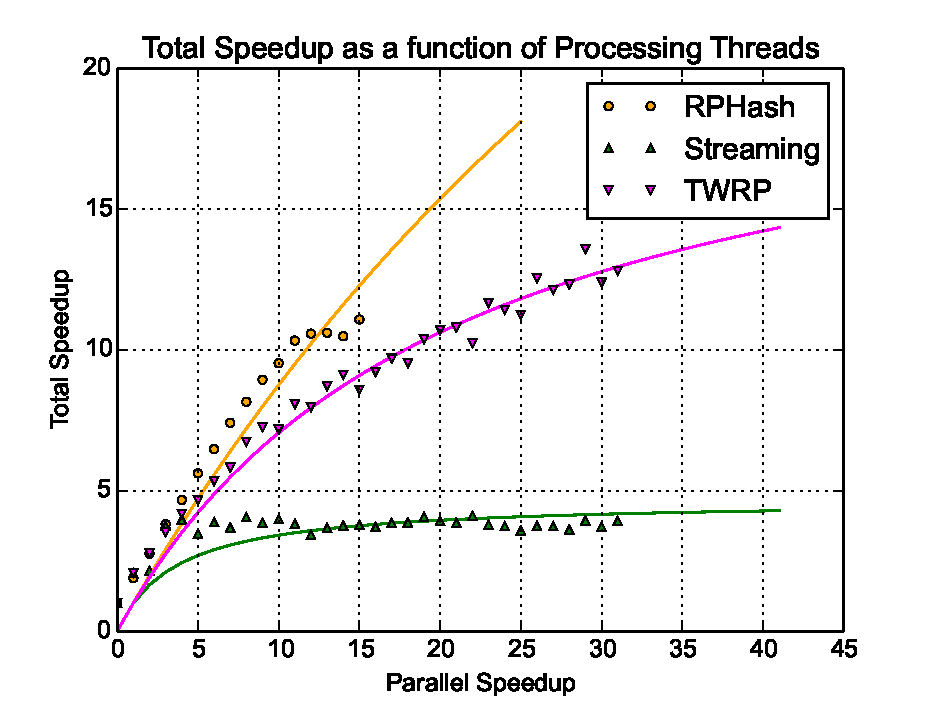
\includegraphics[width=.8\textwidth]{figs/minskispeedup}}
  \caption{Speedup Comparison between RPHash Algorithms}\label{minskispeedup}
\end{figure}

\section{Security Performance}

Due to the inability to anticipate all possible cryptographic attacks on de-anonimization, a
qualitative measure of data obfuscation is developed for comparing a fully qualified vector $v\in
\mathbb{V}^d$ with its corresponding projected vectors $v'\in \mathbb{V}^d$.  This metric referred to
as $k$-anonymity allows us to evaluate the probability of de-anonymization of a vector.

$v'$ is the inverse projection of $u\in \mathbb{V}^s$ that results from the random projection of
$v$.  Destructive data obfuscation occurs if the distance between $v'$ and $v$ is greater than the
distance between $v$ and some other vector $\hat{v}\in \mathbb{V}^d$.  The inverse projection matrix
$R_{d\rightarrow s}^{-1}$ will be used to map $u$ back to $v$'s original subspace.  The two
equations below describe the projection of $v$ to $u$ and the theoretical inverse of the projection
from $u$ to $v'$ under the matrix transform $R_{d\rightarrow s}$ where $d>s$.

$$ u = \sqrt{{\frac{n}{k}}}R_{d\rightarrow s}^Tv $$
$$ v' = \sqrt{{\frac{k}{n}}}u^T R_{d\rightarrow s}^{-1} $$

The above inversion is theoretical however due to the orthogonal projection $R_{d\rightarrow s}$
being non-square and not invertible.  Therefore, for a projection matrix $R_{d\rightarrow s}$ the
least squares solution $\hat{R}_{d\rightarrow s}^{-1}$ will serves as the optimal inverse of the
projection.  Even in the not strictly orthogonal random projection case (as in Achlioptas
\cite{Achlioptas01} and \textsf{RPHash}) the least-squares solution will result in an over-determined
system of equations.  Which implies that any pseudo-inverse projection of a vector in $V^s$ to $V^d$
will result in unrecoverable data loss for non-trivial cases (\emph{i.e.},
$<$\textbf{0}$>$,$<$\textbf{1}$>$).  The goal in testing the security of \textsf{RPHash} is to show
that the data loss is sufficient to make it impossible for an attacker to re-associate the projected
vectors.  A formal definition of the requirement for destructive data obfuscation follows:

$$
s(v,v') = ||v,v'||_{2} 
$$

$$
\forall\{v,v'\} \in V , \exists {\hat{v}} \in V : s(v,v')>s(\hat{v},v) \text{ where }
\hat{v}\neq v ~ \textrm{or} 
$$

$$
Pr(NN((v\cdot R)\cdot \hat{R}^{-1},V)=v)\lesssim {1\over{||V||}}
$$

Due to the often sensitive nature of medical data, we give a real world example based on the MIMIC
II \cite{MIMICII} data set.  Figure \ref{projrecov} shows the $k$-anonymity curve for vector
recoverability demonstrating the effectiveness of random projection for providing vector
anonimization.  The overall bi-clustering in full and reduced dimensions showed little to no
degradation over full and reduced subspaces down to 10 dimensions.  This is further corroborated on
additional data in Bingham \cite{bingham}.  Following the above definition of destructive data
obfuscation, we constructed a test on the MIMIC II data.  The Moore-Penrose inverse generated from
the reciprocal of the singular value decomposition diagonal matrix is generated from the projection
matrix and used as the least squares inverse projection to remap the projected vectors to their
original subspace.  The nearest neighbor method was then used to query the original set of vectors
to see if a vector can be re-associated with itself.  In the results it is clear that as
dimensionality increases, the probability of re-association converges to random coincidence of a
Bernoulli trial $((1-(1/n))^n) \approx .363$.  The successful re-associate rate follows an inverse
power-law like distribution.

\begin{figure}
\centering
 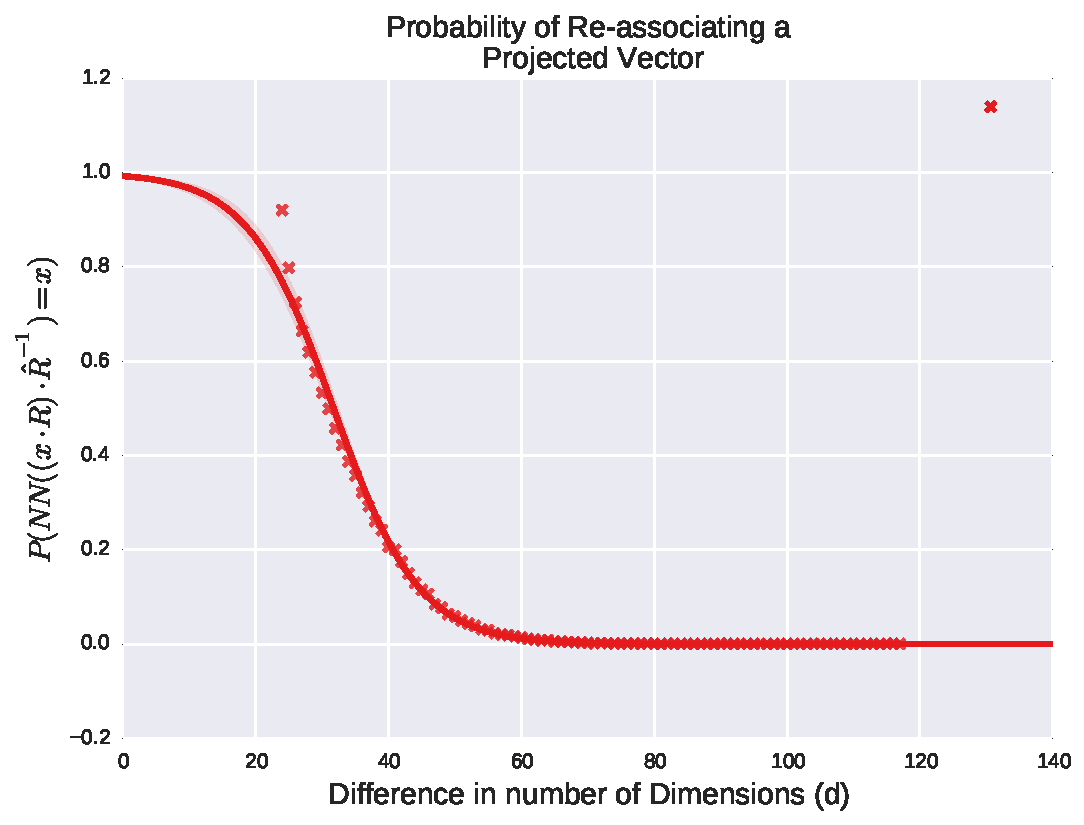
\includegraphics[width=.7\textwidth]{figs/recovery}
  \caption{Probability of Vector Re-association for MIMIC II BioMetric Signatures}\label{projrecov}
\end{figure}

In regard to security performance, it is fairly clear that data becomes unrecoverable when the
difference between the original data embedding and the projected space exceeds 75 dimensions.  Given
that \textsf{RPHash}'s native clustering space is 24 dimensions, this case occurs for a wide variety of high
dimensional datasets, namely those that exceed 99 dimensions.
